\chapter{Resultater og analyse fra Case 2: Kompromitterte brukerkontoer ved NTNU}
I dette kapittelet fremlegger vi våre resultater i alle fasene i case 2.

\section{Problemforståelse}

\subsection{Kritiske hendelser}
Sammen med oppgavebeskrivelsen fikk vi en liste over loggførte sikkerhetshendelser som hadde foregått det siste året hvor kompromitterte kontoer var involvert. Dataene ble sortert i synkende rekkefølge og lagt inn i en tabell for å visualisere frekvensen til de enkelte sikkerhetshendelsene, og dermed fokusområdene til trusselaktørene. 

\begin{table} [H]
    \begin{tabular}{ | m{18em} | m{18em} | }
        \hline
            \cellcolor{yellow} Sikkerhetshendelser & \cellcolor{yellow} Frekvens \\
        \hline
            Spam & 46  \\
        \hline
            Misuse (uthenting av forskningsartikler) & 26 \\
        \hline
            Negligible/Fixed/Failed Attack  & 8 \\
        \hline
            Phishing & 7 \\
        \hline
            Whaling & 2 \\
        \hline
            Brute force & 2 \\
        \hline
            DDOS out & 1 \\
        \hline
            Traded credentials & 1 \\
        \hline
            Hackingtools exploits and kits & 1 \\
        \hline
            Copyright/Piracy & 1 \\
        \hline
    \end{tabular}
    \caption{Oversikt over hva kompromitterte ansattkontoer blir brukt til}
    \label{kritisk_tabell_2}
\end{table}

Fra tabellen ser vi at spam er den hendelsen med høyest frekvens, men etter diskusjon med oppdragsgiver var ikke dette problemet av størst viktighet. Det er fordi dette er noe som enkelt blir lagt merke til og er trolig ikke hovedgrunnen til at aktørene aktivt går inn for å kompromittere NTNU sine brukerkontoer. Når det kommer til ``misuse'' i tabellen ovenfor referer det til hendelser der uvedkommende misbruker NTNU sine ressurser, spesielt i form av å stjele forskningsartikler på NTNU sin regning. Dette var en av de største problemene med kompromittering av kontoene, siden det førte til økonomisk tap for NTNU og fare for utestengelse fra artikkeldatabasene. 

\section{Idémyldring}
I denne fasen ble det gjort en idémyldring. Problemet som ble fremhevet var hvordan brukerkontoer ble kompromittert. Resultatet fra idémyldringen, gruppert i henhold til likhetstrekk, vises i figur \ref{fig:case2-idemyldring} under. 

\begin{figure}[H]
    \centering
    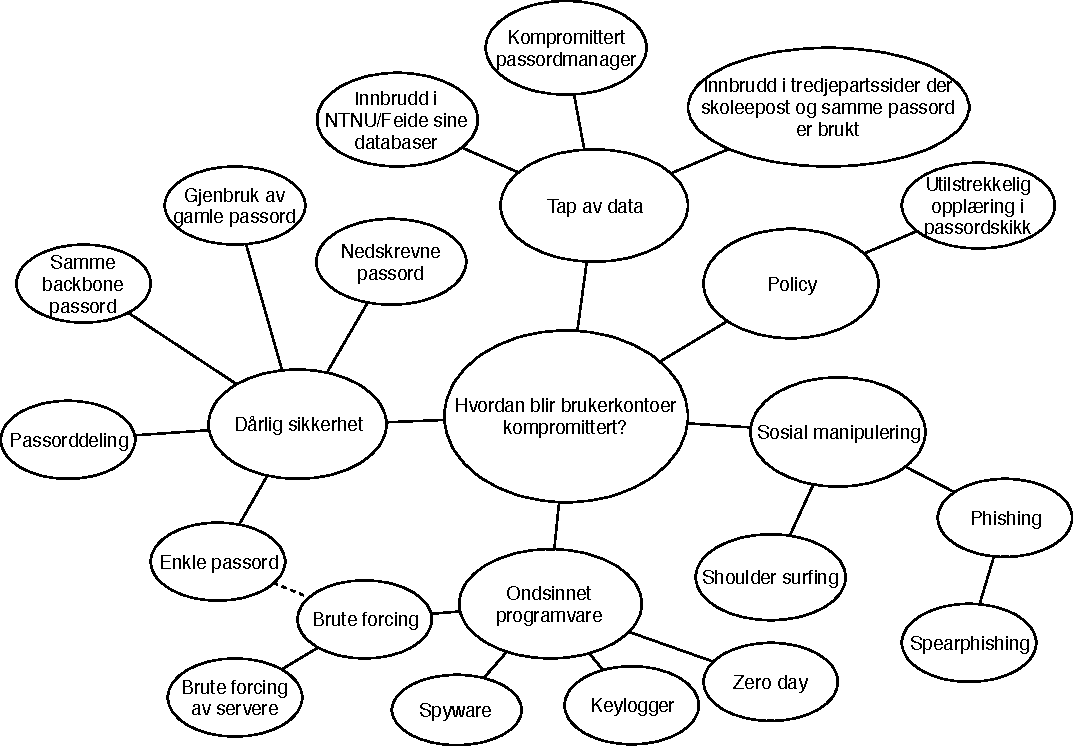
\includegraphics[scale=0.6]{case_2/bilder/idemyldring.pdf}
    \caption[Idémyldring for kompromitterte kontoer]{Resultater og gruppering av idémyldringen}
    \label{fig:case2-idemyldring}
\end{figure}

Resultatene er gruppert inn i 4 hovedkategorier:
\begin{description}
    \item [Dårlig sikkerhet] er alt fra enkle passord til passordgjenbruk.
    \item [Tap av data] inkluderer at for eksempel sider som dropbox har en lekkasje av brukerinformasjon.
    \item [Sosial manipulering] vil si å få tak i informasjon ved å lure noen.
    \item [Ondsinnet programvare] er programvare brukt som hjelpemiddel for å få tak i brukerinformasjon.
\end{description}

\section{Datainnsamling}
Under idémyldringen ble det avdekket en rekke faktorer som kunne være medvirkende i at ansatte og studenter ved NTNU fikk sin konto på avveie. Vi brukte denne informasjonen aktivt da spørreundersøkelsen ble konstruert. Spørreundersøkelsen slik den fremstår for respondenten finnes i vedlegg \ref{undersokelse_norsk}. Når spørsmålene ble laget ble det bestemt hypoteser til spørsmålene. Disse er listet i tabell \ref{tab:case2-hypoteser} under. 

% Table generated by Excel2LaTeX from sheet 'Ark2'
\begin{table}[H]
  \centering
  \caption{Hypoteser til spørsmålene for kompromitterte kontoer}
    \begin{tabular}{|p{20.215em}|p{20.57em}|}
    \hline
    \rowcolor{yellow} Spørsmål & Hypoteser \\
    \hline
    Din alder? & Eldre er overrepresentert i statistikken over tapte kontoer \\
    \hline
    Ditt kjønn? & Flere kvinner enn menn har blitt kompromittert \\
    \hline
    Hva er din primærrolle ved NTNU? & Det er ansatte som er målgruppen til trusselaktørene \\
    \hline
    I hvilken by jobber/studerer du primært? & Gjøvik har høyere sikkerhetskompetanse \\
    \hline
    I hvor mange år har du jobbet/studert ved NTNU eller de tidligere høgskolene? & Folk med lavere ansiennitet kjenner universitetets retningslinjer bedre \\
    \hline
    Når fant du ut at NTNU kontoen din var blitt kompromittert? & Folk vet ikke at de har blitt kompromittert før de blir kontaktet \\
    \hline
    Har du noen formening om hvor lang tid kontoen var kompromittert før Seksjon for Digital Sikkerhet kontaktet deg? & Ingen hypotese grunnet vagt spørsmål \\
    \hline
    Har du noen formening om hvordan kontoen din ble kompromittert? & Ingen hypotese grunnet åpent svar \\
    \hline
    Bruker du din NTNU e-post til å registrere deg på ulike tjenester på nett i forbindelse med jobben/studiet? & Over halvparten bruker NTNU e-post til tjenester i forbindelse med jobb \\
    \hline
    Bruker du din NTNU e-post til å registrere deg på tjenester på nett til privat bruk? & Under halvparten bruker NTNU e-post til privat bruk \\
    \hline
    På en skala fra 1-6, der 1 er lite bevisst og 6 er svært bevisst, hvor bevisst er du på sikkerhet når du... & \multirow{4}[2]{*}{Folk er generelt sett lite bevisste} \\
    besøker nettsider? & \multicolumn{1}{r|}{} \\
    lager passord? & \multicolumn{1}{r|}{} \\
    sjekker e-post? & \multicolumn{1}{r|}{} \\
    \hline
    Har du i din tid hos NTNU lagt merke til phishing-forsøk mot deg på din NTNU e-post? & Phishing er en svært utbredt angrepsvektor \\
    \hline
    Har du blitt lurt av phishing på din NTNU e-post? & Av de som har blitt kompromittert har under en tredjedel blitt lurt av phishing \\
    \hline
    Har du i løpet av din tid ved NTNU eller de andre høgskolene, oppdaget virus eller annen skadevare på maskinen din? & Virus og annen skadevare er utbredt \\
    \hline
    Bruker du ditt NTNU passord på flere tjenester? & Passordgjenbruk er utbredt \\
    \hline
    Brukte du regler til å generere ditt NTNU passord? & De fleste bruker ikke passordregler til å generere passord \\
    \hline
    Er ditt NTNU passord tilfeldig sammensatt av bokstaver, tall og/eller tegn? & De fleste bruker ikke tilfeldig sammensatte passord \\
    \hline
    Hvor mange tegn består ditt NTNU passord av? & Over halvparten har passord på under 12 tegn \\
    \hline
    Har du i løpet av din tid ved NTNU delt NTNU passordet ditt med andre? & Passorddeling er ikke særlig utbredt \\
    \hline
    Omtrent hvor ofte bytter du ditt NTNU passord? & Passord byttes for det meste sjeldnere enn hvert andre år \\
    \hline
    Bruker du en passordmanager? & De fleste bruker ikke passordmanager, og mange vet ikke engang hva det er \\
    \hline
    På en skala fra 1 til 6, hvor godt kjent er du med... & \multirow{4}[2]{*}{Det er svært lite kjennskap til retningslinjer} \\
    NTNU sine retningslinjer for behandling av brukernavn, passord og andre autentiseringsdata? & \multicolumn{1}{r|}{} \\
    IT-reglementet til NTNU? & \multicolumn{1}{r|}{} \\
    NTNU sine prinsipper for informasjonssikkerhet? & \multicolumn{1}{r|}{} \\
    \hline
    Har du fått opplæring i passordsikkerhet fra NTNU? & Under en fjerdedel har fått opplæring i passordskikk fra NTNU \\
    \hline
    \end{tabular}%
  \label{tab:case2-hypoteser}%
\end{table}%

Av de som e-posten ble sendt ut til fikk vi totalt 72 gyldige respondenter, mens 26 stoppet rett etter åpning av undersøkelsen eller underveis. Undersøkelsen var aktiv i perioden fra 20. April til og med 27. April. I løpet av denne tiden ble det sendt ut én purring den 25. April. 

\section{Dataanalyse}
I denne fasen analyseres dataene som er samlet inn, og ved hjelp av statistiske verktøy kan vi trekke konklusjoner basert på svarene. Verktøyet vi bruker til å utføre mesteparten av analysene er SPSS.

\subsection{Svarstatistikk}
Spørreundersøkelsen ble mottatt av 157 personer som har fått kontoen kompromittert. Av disse var det 72 som svarte. Det var i tillegg 26 som startet spørreundersøkelsen, men ikke fullførte. Figur \ref{fig:case2-svar-per-dag} under viser statistikk over hvor mange svar som kom inn per dag.

\begin{figure}[H]
    \centering
    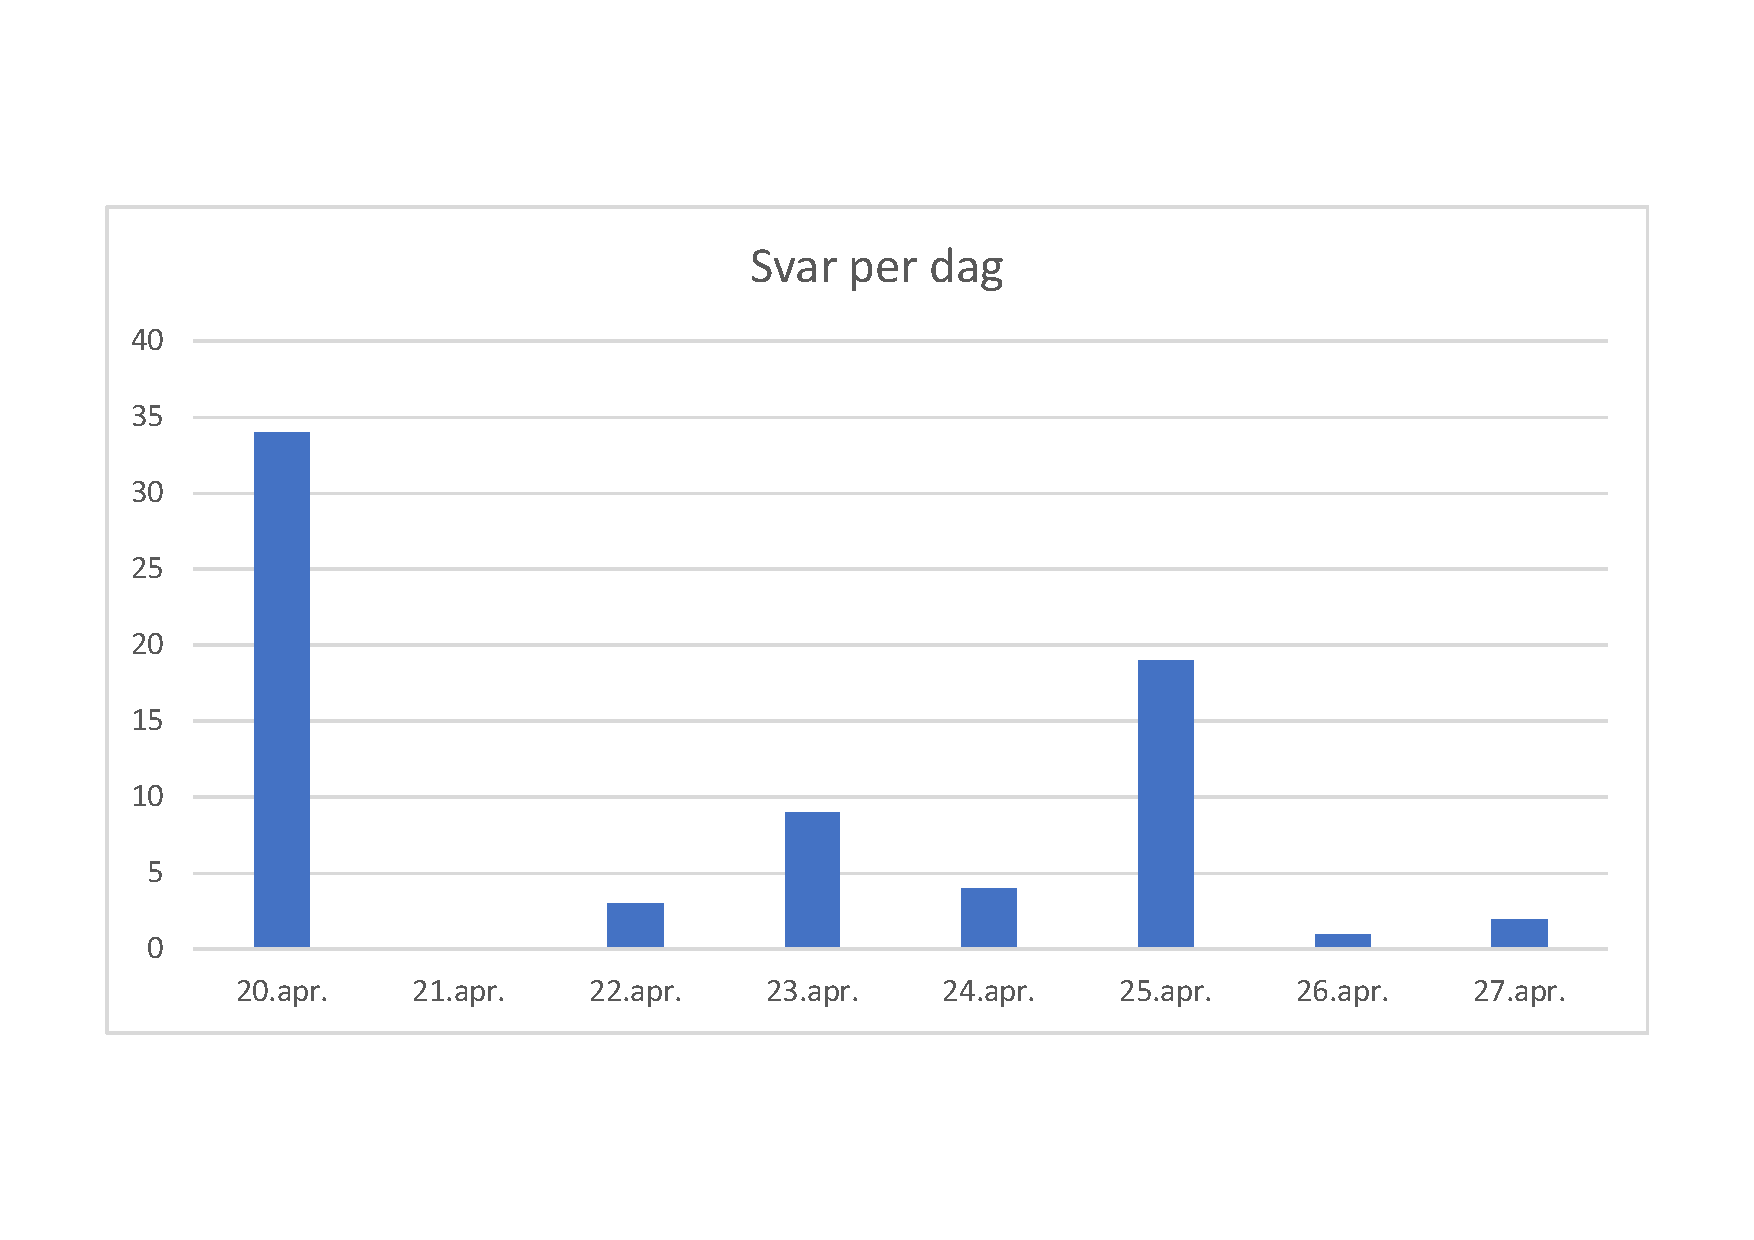
\includegraphics[scale=0.5, clip, trim=1cm 3cm 0cm 3cm]{case_2/bilder/spss/svar_per_dag.pdf}
    \caption[Svar per dag]{Antall svar vi fikk per dag}
    \label{fig:case2-svar-per-dag}
\end{figure}

Det var tydelig mest svar dagen spørreundersøkelsen ble lansert, og 25. April, hvor vi sendte ut en purre e-post. Det bør nevnes at undersøkelsen ble sendt ut på en fredag, og 21. og 22. April var en lørdag og søndag. Derfor gikk antall svar litt opp igjen på mandag 23. April. 

\subsection{Demografi}
I denne delen fremlegges resultatene fra demografien i spørreundersøkelsen. Disse blir om mulig sammenliknet med generelle tall fra NTNU for å få et innblikk i demografien til de som har blitt kompromittert, kontra NTNU sine ansatte og studenter generelt. Vi fokuserer stort sett på de ansatte siden antall studenter i undersøkelsen var få.

\subsubsection{Aldersgruppe}
Aldersgruppene ble kategorisert i intervaller på 10 år. Fra de ulike kategoriene fikk vi:

\begin{itemize}
    \item Under 20: 1 person
    \item 20-29: 3 personer
    \item 30-39: 13 personer
    \item 40-49: 27 personer
    \item 50-59: 11 personer
    \item 60-69: 9 personer
    \item 70 eller over: 8 personer
\end{itemize}

Under ser vi aldersfordelingen visuelt fremstilt i et histogram.

\begin{figure}[H]
    \centering
    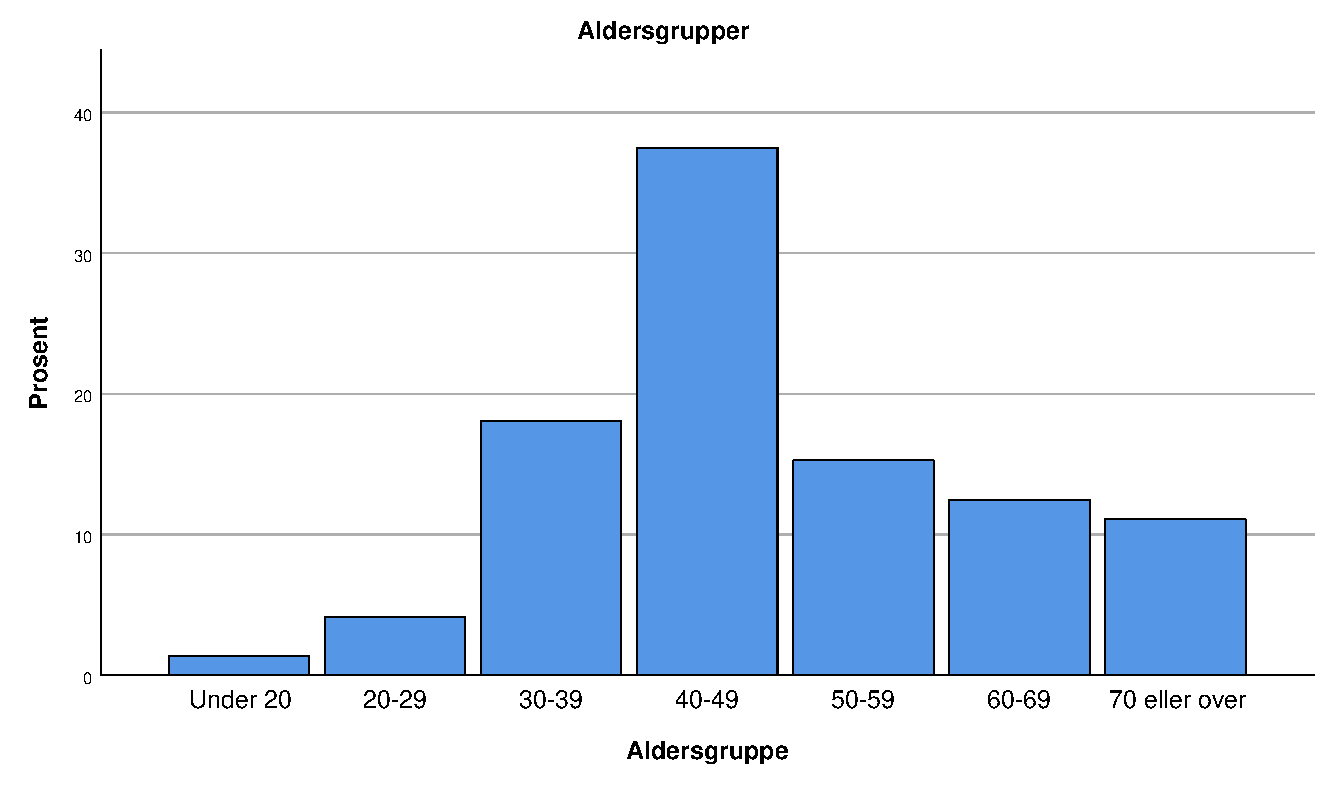
\includegraphics[scale=0.5]{case_2/bilder/spss/aldersgrupper.pdf}
    \label{fig:case2-aldersgruppe}
    \caption[Aldersgrupper av de kompromitterte]{Aldersgrupper av respondentene}
\end{figure}

Ut fra resultatene kan vi konkludere med at de som har blitt kompromittert er stort sett middelaldrene til eldre personer. Disse personene er også noe eldre enn gjennomsnittsalderen til de som jobber ved NTNU \cite{MorkRapport}. 

\subsubsection{Kjønn}
Av de 72 respondentene var det 45 kvinner og 27 menn. Det er henholdsvis 62,5\% og 37,5\%. Under er kjønnsfordelingen visualisert i et sektordiagram.

\begin{figure}[H]
    \centering
    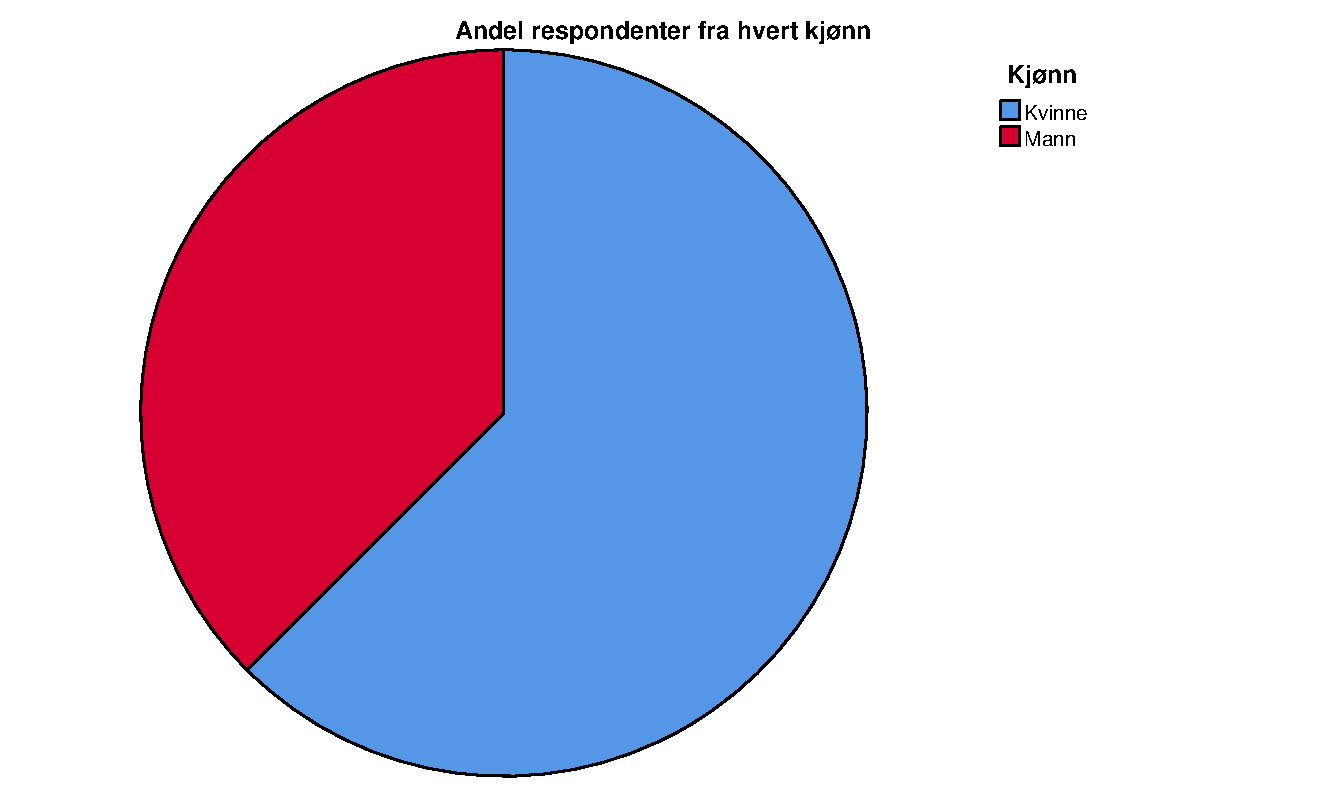
\includegraphics[scale=0.5]{case_2/bilder/spss/kjonn.pdf}
    \label{fig:case2-kjonn}
    \caption[Andel fra hvert kjønn av de kompromitterte]{Andel fra hvert kjønn}
\end{figure}

De fleste av de som har svart er kvinner. Av de ansatte ved NTNU er det 41\% kvinner totalt \cite{NTNUfakta}. Totalt sendte vi ut spørreundersøkelsen til 167 e-postadresser, der 157 av de mottok. Vi har tall på at 91 av de 167 vi først sendte ut til var kvinner. Dette er omtrent 55\%. For å kunne si noe om antallet kvinner som svarte på spørreundersøkelsen må vi se på om svarene våre er representative for hele samplet. Vi brukte en kalkulator for å regne ut konfidensintervallet for vårt sample \cite{SSCalc}. Utregningen kom fram til at vi er 95\% sikre på at feilmarginen for dette spørsmålet er \(\pm 8,5\%\). I og med at andelen kvinner totalt på NTNU er 41\%, kan vi fastslå at kvinner er noe mer utsatt for å få kontoen kompromittert, men denne forskjellen er ikke stor.

\subsubsection{Primærrolle}
Av de 72 respondentene var det 6 studenter og 66 ansatte. Dette er henholdsvis 8,3\% og 91,7\%. Sektordiagrammet under viser fordelingen.

\begin{figure}[H]
    \centering
    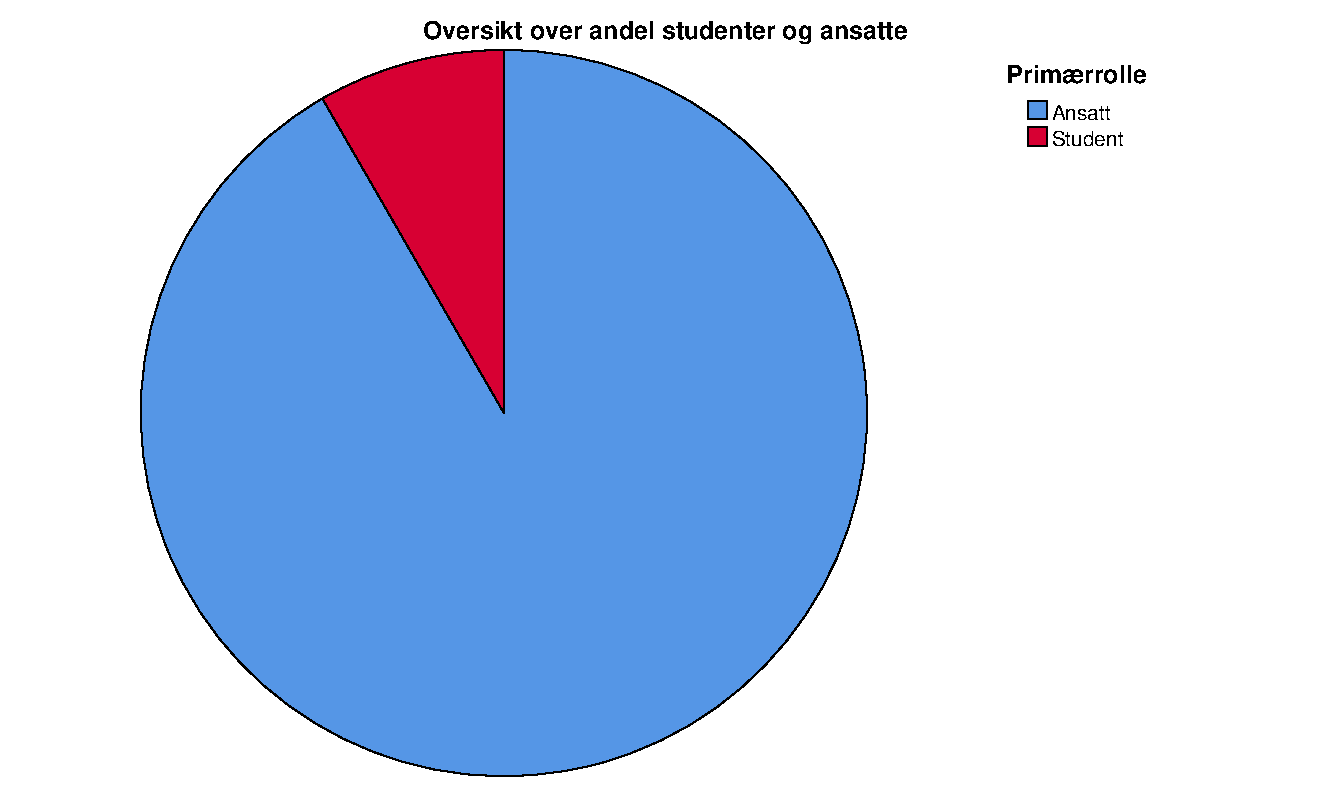
\includegraphics[scale=0.5]{case_2/bilder/spss/primaerrolle.pdf}
    \label{fig:case2-primaerrolle}
    \caption[Primærrolle ved NTNU]{Primærrolle ved NTNU}
\end{figure}

Fra dataene kan vi se at ansatte er overrepresentert i de som blir kompromittert. Vi har data på at det er 18 studenter i vårt sample, altså står studenter for omtrent 10\% av de kompromitterte. På samme måte som i forrige seksjon, ble konfidensintervallet regnet ut \cite{SSCalc}. Utregningen kom frem til at vi er 95\% sikre på at feilmarginen er på \(\pm 5,12\%\). Det er desidert flere studenter enn ansatte ved NTNU \cite{NTNUfakta}. Derfor kan vi med høy sikkerhet si at trusselaktørenes målgruppe er de ansatte og ikke studenter. 

\subsubsection{Primærby}
Av de 72 respondentene var det bare en fra Ålesund og resten var fra Trondheim. Det var ingen respondenter fra Gjøvik. 

\subsubsection{År ved NTNU}
Bare 6 personer, eller 8,3\% av respondentene hadde jobbet eller studert ved NTNU i under 2 år og i 2 til 4 år. 9 personer, eller 12,5\% hadde jobbet eller studert her i 5 til 9 år, og 15 personer, eller 20,8\% hadde jobbet eller studert her i 10 til 15 år. Hele 36 personer, eller akkurat halvparten av respondentene har vært hos NTNU i over 15 år. En oversikt over disse tallene finnes i histogrammet under. 

\begin{figure}[H]
    \centering
    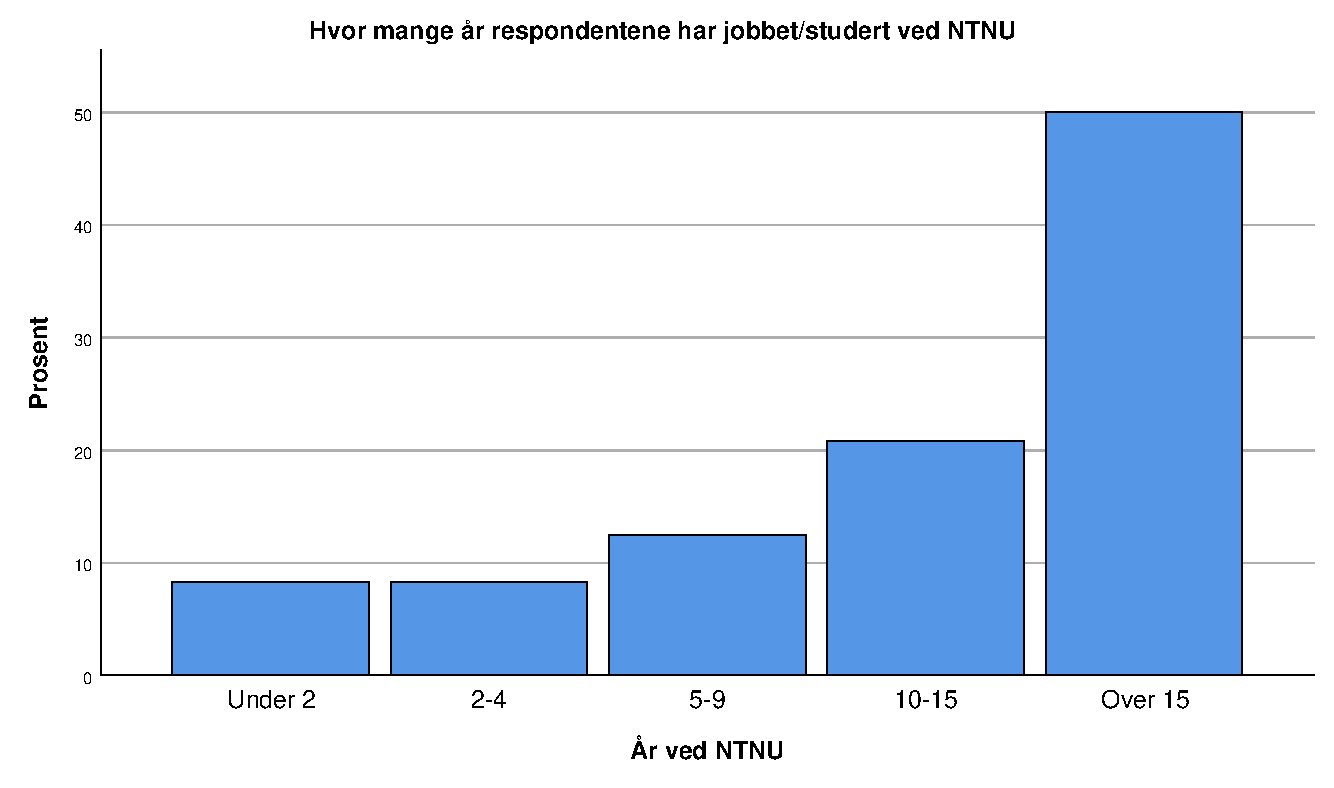
\includegraphics[scale=0.5]{case_2/bilder/spss/aarvedNTNU.pdf}
    \label{fig:case2-aarvedNTNU}
    \caption[Antall år ved NTNU]{Antall år ved NTNU}
\end{figure}

\subsection{Bevissthet på sikkerhet}
Spørsmålene skulle gi svar på hvor sikkerhetsbevisst en tenker når man besøker nettsider, lager passord og sjekker e-post. Hypotesen som ble fremhevet her var at folk generelt sett er lite bevisste. 

Histogrammet i figur \ref{fig:case2-bevisst-nettsider} viser en tilnærmet normalfordelt situasjon, men med noe fler svar på høyresiden. De fleste er derfor litt mer bevisste på sikkerhet når de besøker nettsider enn de er ubevisste. 
\begin{figure}[H]
    \centering
    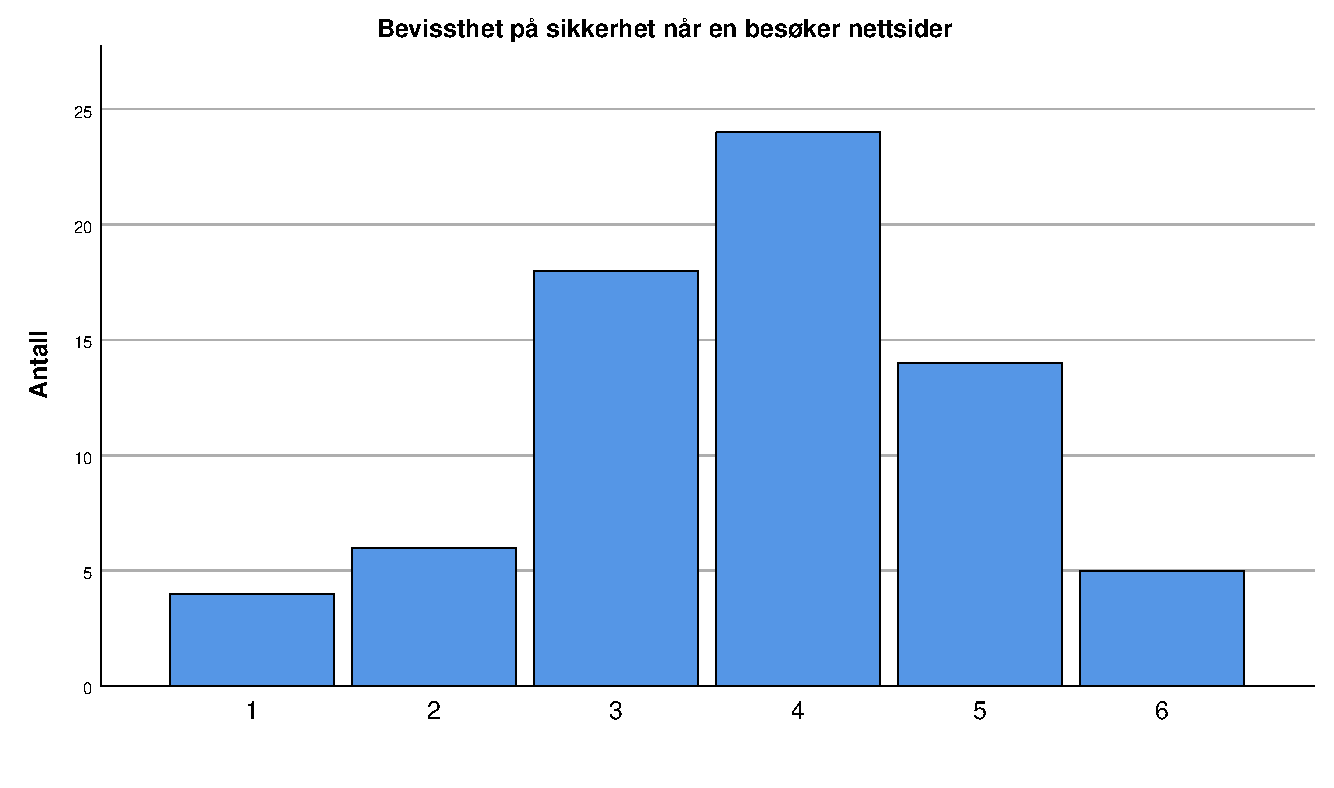
\includegraphics[scale=0.5]{case_2/bilder/spss/bevisst_nettsider.pdf}
    \caption[Bevisst på sikkerhet med nettsider]{Bevissthet på sikkerhet når en besøker nettsider}
    \label{fig:case2-bevisst-nettsider}
\end{figure}

Når det kommer til sikkerhet når en lager passord svarer respondentene at de generelt sett er bevisste på dette. Figur \ref{fig:case2-bevisst-passord} under viser at fordelingen er konsentrert hovedsaklig på høyresiden.
\begin{figure}[H]
    \centering
    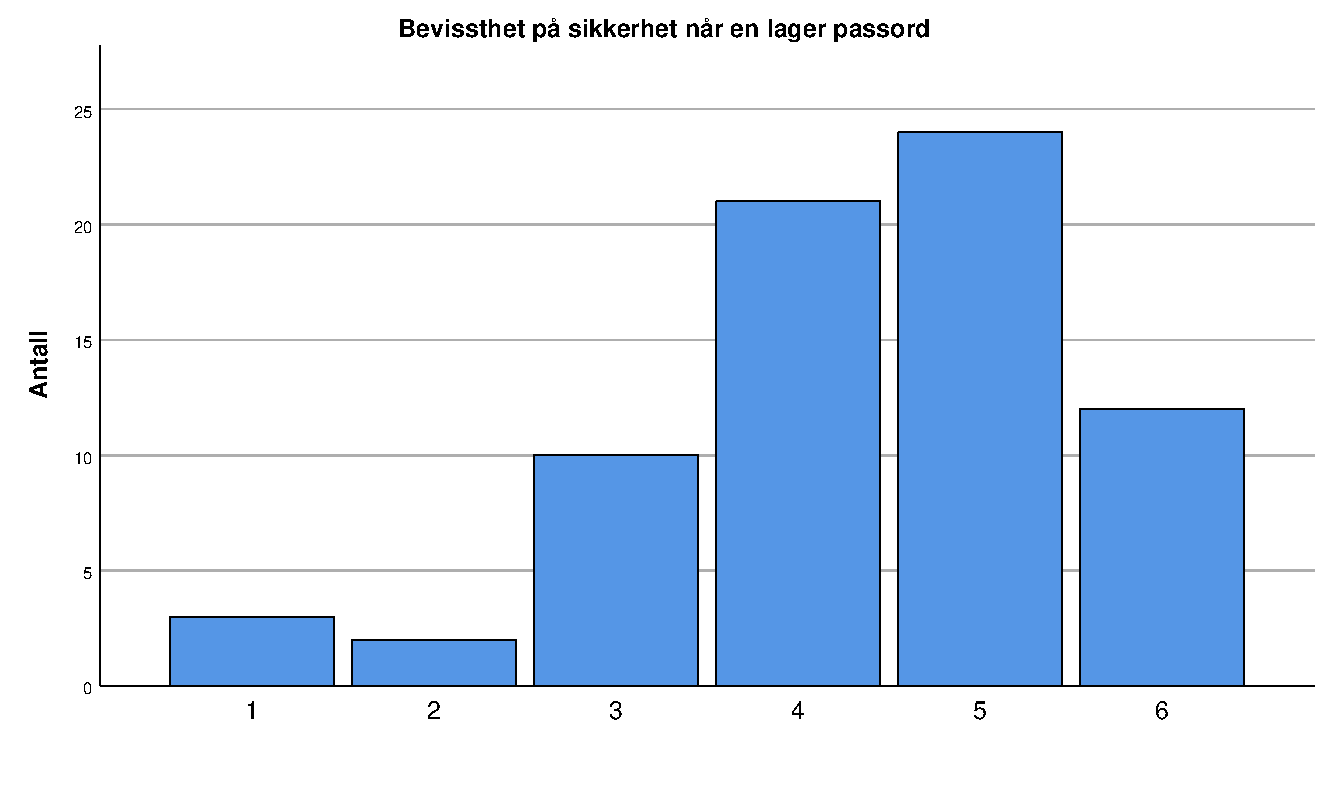
\includegraphics[scale=0.5]{case_2/bilder/spss/bevisst_passord.pdf}
    \caption[Bevisst på sikkerhet med passord]{Bevissthet på sikkerhet når en lager passord}
    \label{fig:case2-bevisst-passord}
\end{figure}

Figur \ref{fig:case2-bevisst-e-post} under viser bevissthetsfordelingen når det kommer til sjekking av e-post. Dette var noe vi spesielt ønsket å se på siden en av hovedhypotesene våre til kompromitterte brukerkontoer er phishing. Histogrammet viser at respondentene stort sett er bevisste på sikkerhet når de sjekker e-post.
\begin{figure}[H]
    \centering
    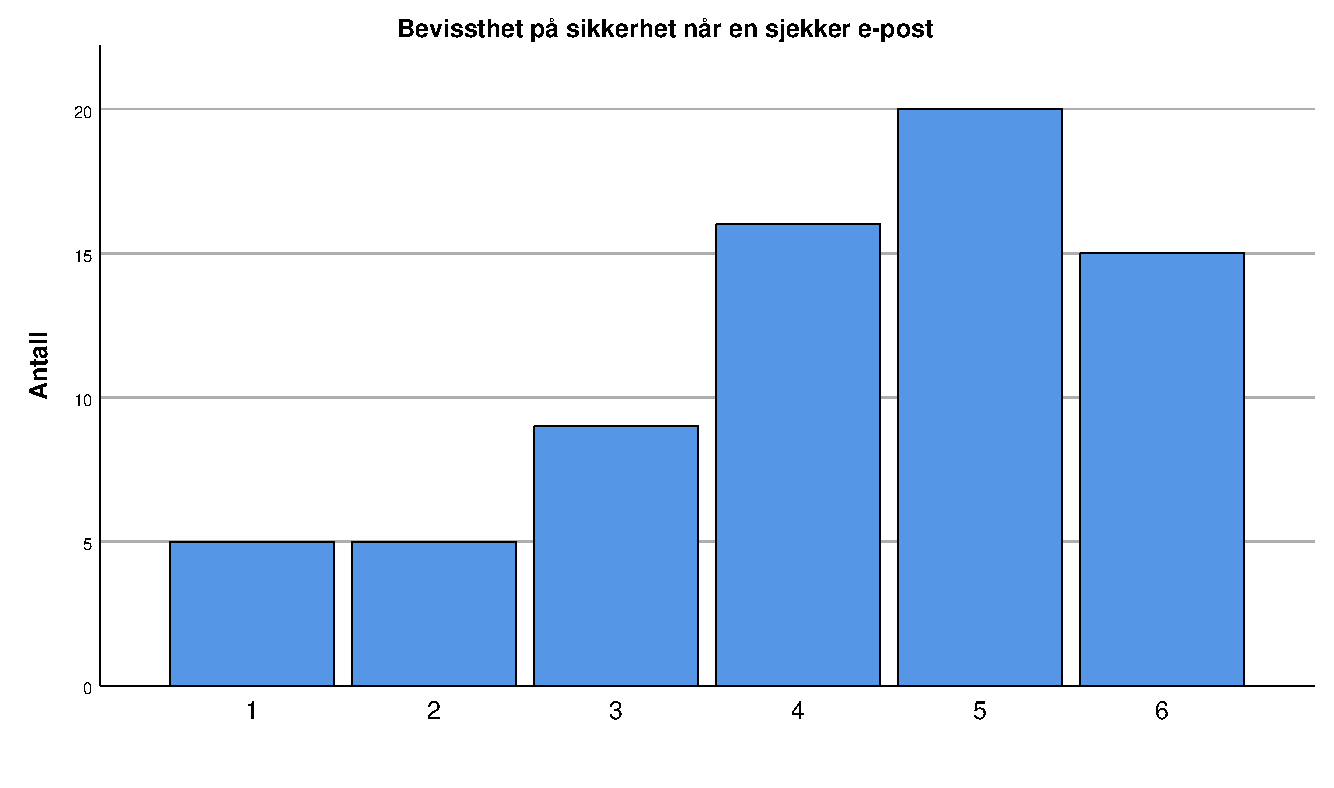
\includegraphics[scale=0.5]{case_2/bilder/spss/bevisst_e-post.pdf}
    \caption[Bevisst på sikkerhet med e-post]{Bevissthet på sikkerhet når en sjekker e-post}
    \label{fig:case2-bevisst-e-post}
\end{figure}

\subsection{Kjennskap til retningslinjer, reglementer og prinsipper}
Disse spørsmålene handler om hvor godt kjennskap respondentene har til NTNU sine retningslinjer for behandling av autentiseringsdata, IT-reglementet og prinsipper for informasjonssikkerhet. Hypotesen vi hadde her var at de aller fleste hadde lite kjennskap til disse.

Det viser seg fra figur \ref{fig:case2-retningslinjer} at respondentene kan lite om NTNU sine retningslinjer for behandling av brukernavn, passord og andre autentiseringsdata. 
\begin{figure}[H]
    \centering
    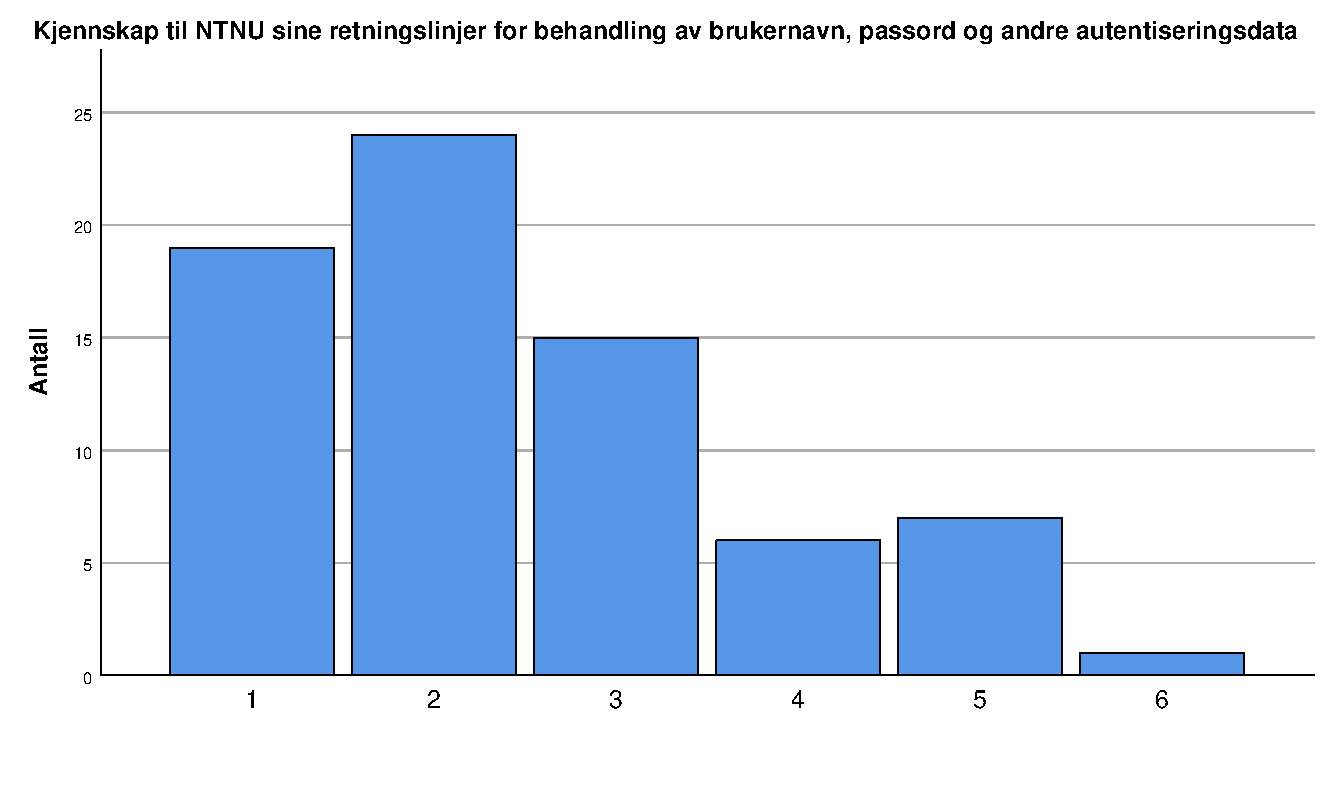
\includegraphics[scale=0.5]{case_2/bilder/spss/retningslinjer.pdf}
    \caption[Kjennskap til retningslinjer]{Kjennskap til retningslinjer}
    \label{fig:case2-retningslinjer}
\end{figure}

Figur \ref{fig:case2-ITreglement} viser at respondentene ikke kjenner så godt til IT-reglementet til NTNU. Over 70\% svarte 3 eller under på hvor godt de kjente IT-reglementet til NTNU, der 1 var lite kjent og 6 var meget kjent.  
\begin{figure}[H]
    \centering
    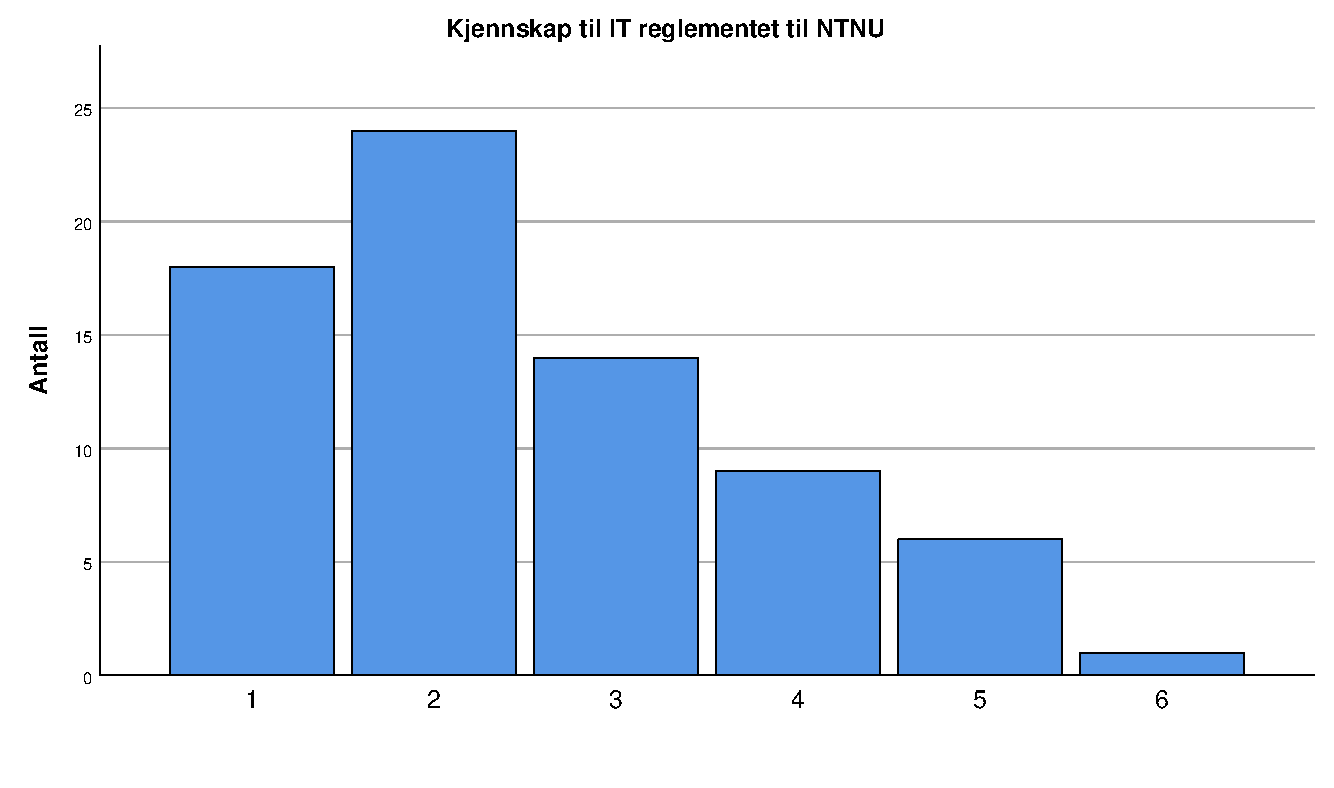
\includegraphics[scale=0.5]{case_2/bilder/spss/ITreglement.pdf}
    \caption[Kjennskap til IT-reglement]{Kjennskap til IT-reglement}
    \label{fig:case2-ITreglement}
\end{figure}

Under viser figur \ref{fig:case2-InfoSecPolicy} at folk har dårlig kjennskap til NTNU sine prinsipper for informasjonssikkerhet. Der står det blant annet at brukere er ansvarlige for enhver bruk av innloggingskredentialier og at de holder dette konfidensielt \cite{PrinsInfoSec}. 
\begin{figure}[H]
    \centering
    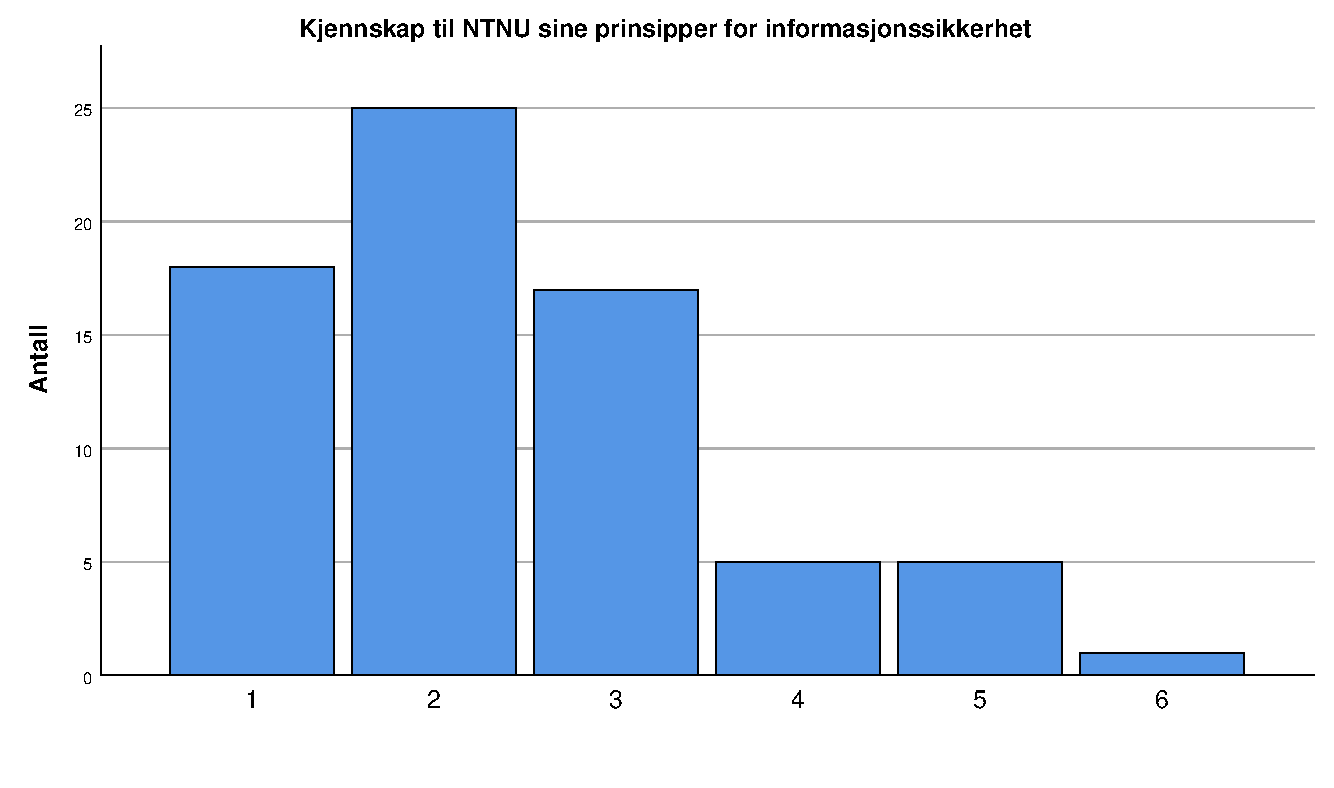
\includegraphics[scale=0.5]{case_2/bilder/spss/InfoSecPolicy.pdf}
    \caption[Kjennskap til prinsipper for informasjonssikkerhet]{Kjennskap til NTNU sine prinsipper for informasjonssikkerhet}
    \label{fig:case2-InfoSecPolicy}
\end{figure}

Det viser seg at hypotesen vi hadde stemte. Det er lite kjennskap til styringsdokumentene.

\subsection{Respondentenes egen oversikt}
Over 60\% av respondentene viste ikke at kontoen var blitt kompromittert før Seksjon for Digital Sikkerhet ringte, og kun 20\% svarte at de fant ut av det før og resten svarte at de ikke vet.

\begin{figure}[H]
    \centering
    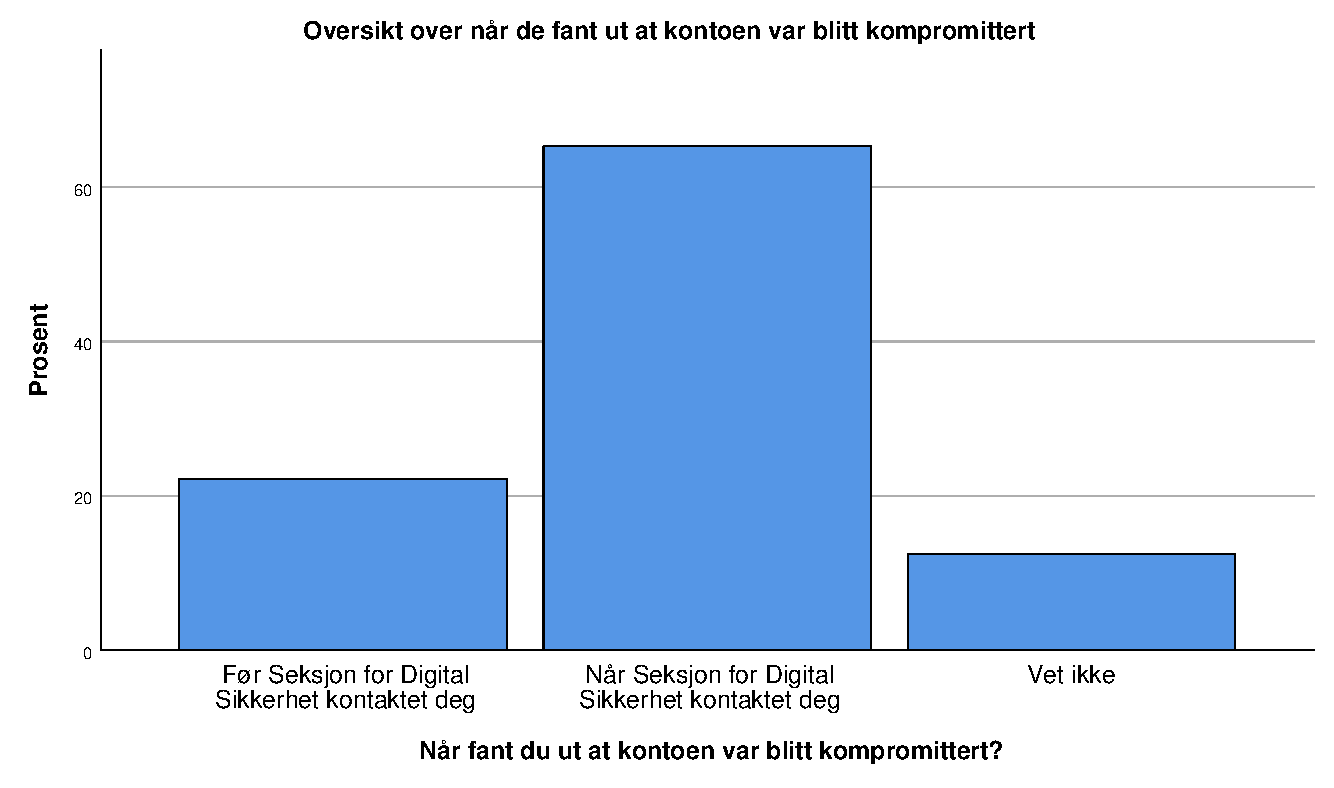
\includegraphics[scale=0.5]{case_2/bilder/spss/Fant_ut_kompromittert.pdf}
    \caption[Når de fant ut de var kompromittert]{Viser når de fant ut at de var blitt kompromittert}
    \label{fig:case2-fant-ut-kompromittert}
\end{figure}

Hypotesen vår her var korrekt. De vet ikke at de har blitt kompromittert før de blir kontaktet.

Respondentene svarte at de trodde kontoen var kompromittert mindre enn tre måneder før Seksjon for Digital Sikkerhet kontaktet dem, som vist i figur \ref{fig:fant-ut-kompromittert}. Denne statistikken kan vi ikke være helt sikre på, fordi halvveis i undersøkelsen fikk vi tilbakemeldiner på at det var flere som ikke ville fullføre spørreundersøkelsen siden dette svaret var obligatorisk og det ikke var noe alternativ for ``vet ikke''. Vi fjernet da kravet om å svare halvveis ut i undersøkelsen.
\begin{figure}[H]
    \centering
    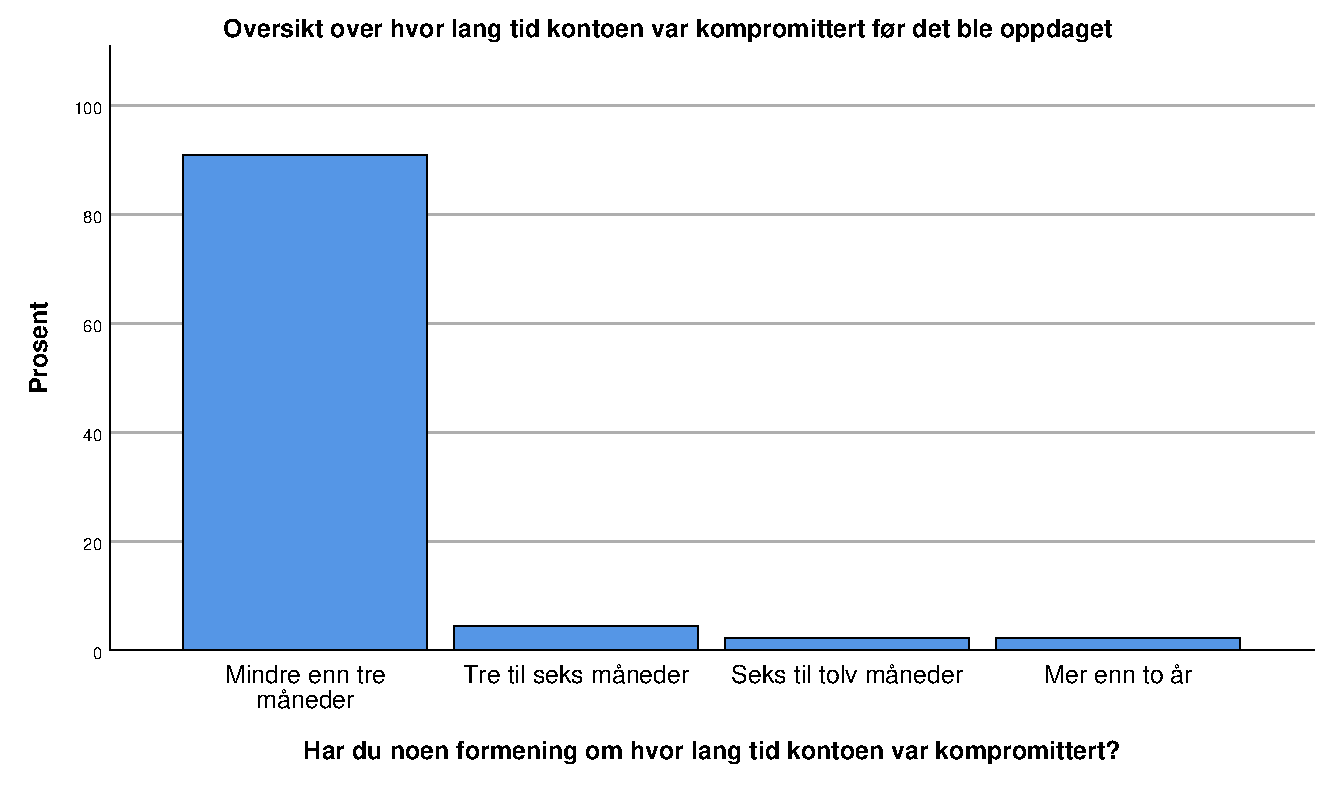
\includegraphics[scale=0.5]{case_2/bilder/spss/lang_tid_konto_kompromittert.pdf}
    \caption[Hvor lang tid de tror de var kompromittert]{Viser hvor lang tid de tror de var kompromittert}
    \label{fig:fant-ut-kompromittert}
\end{figure}

\subsubsection{Formening om hvordan det skjedde}
Affinitetsdiagramet viser at 62 av respondentene ikke har noen formening om hvordan kontoen ble kompromittert. Det var fire som trodde det skjedde på grunn av phishing og tre som trodde det var på grunn av at en annen tjeneste ble hacket eller utdatert programvare. I tillegg var det bare en som svarte at passordgjenbruk var problemet, og samme antall svarte at det var virus. 
\begin{figure}[H]
    \centering
    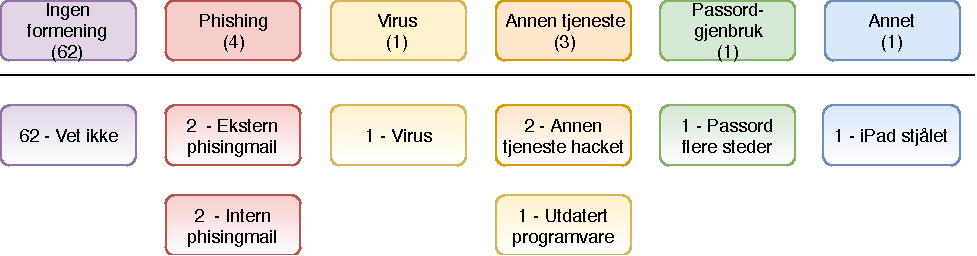
\includegraphics[scale=0.8]{case_2/bilder/Affinitetsdiagram.pdf}
    \caption[Affinitetsdiagram av formening om hvordan det skjedde]{Affinitetsdiagram av respondentenes formening over hvordan kontoen ble kompromittert}
    \label{fig:case2-affinitetsdiagram}
\end{figure}

\subsection{Bruker- og passordvaner}
Som vi kan se i figur \ref{fig:case2-epost-jobb} under, bruker over 60\% av respondentene NTNU e-posten til å registrere seg på tjenester i forbindelse med jobb.
\begin{figure}[H]
    \centering
    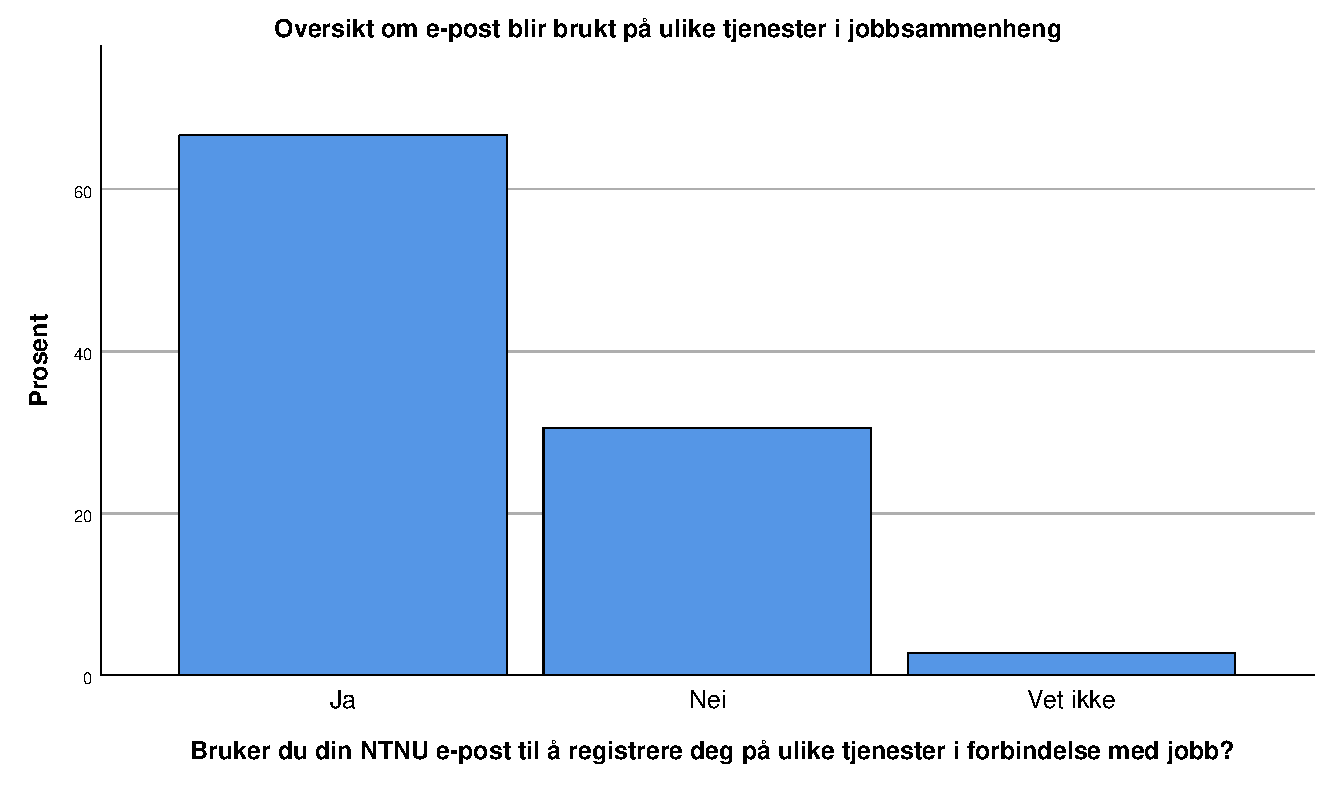
\includegraphics[scale=0.5]{case_2/bilder/spss/epost_jobb.pdf}
    \caption[E-post til jobbrelaterte tjenester]{Viser hvor mange som bruker NTNU e-post til andre jobbrelaterte tjenester}
    \label{fig:case2-epost-jobb}
\end{figure}
Hypotesen vår var korrekt, over halvparten bruker NTNU e-posten i forbindelse med jobb. 

48,6\% av respondentene bruker NTNU e-posten sin til private tjenester. Den samme andelen gjør ikke det og de restende (2,8\%) har svart at de ikke vet. Dette blir vist i figur \ref{fig:case2-epost-privat}.
\begin{figure}[H]
    \centering
    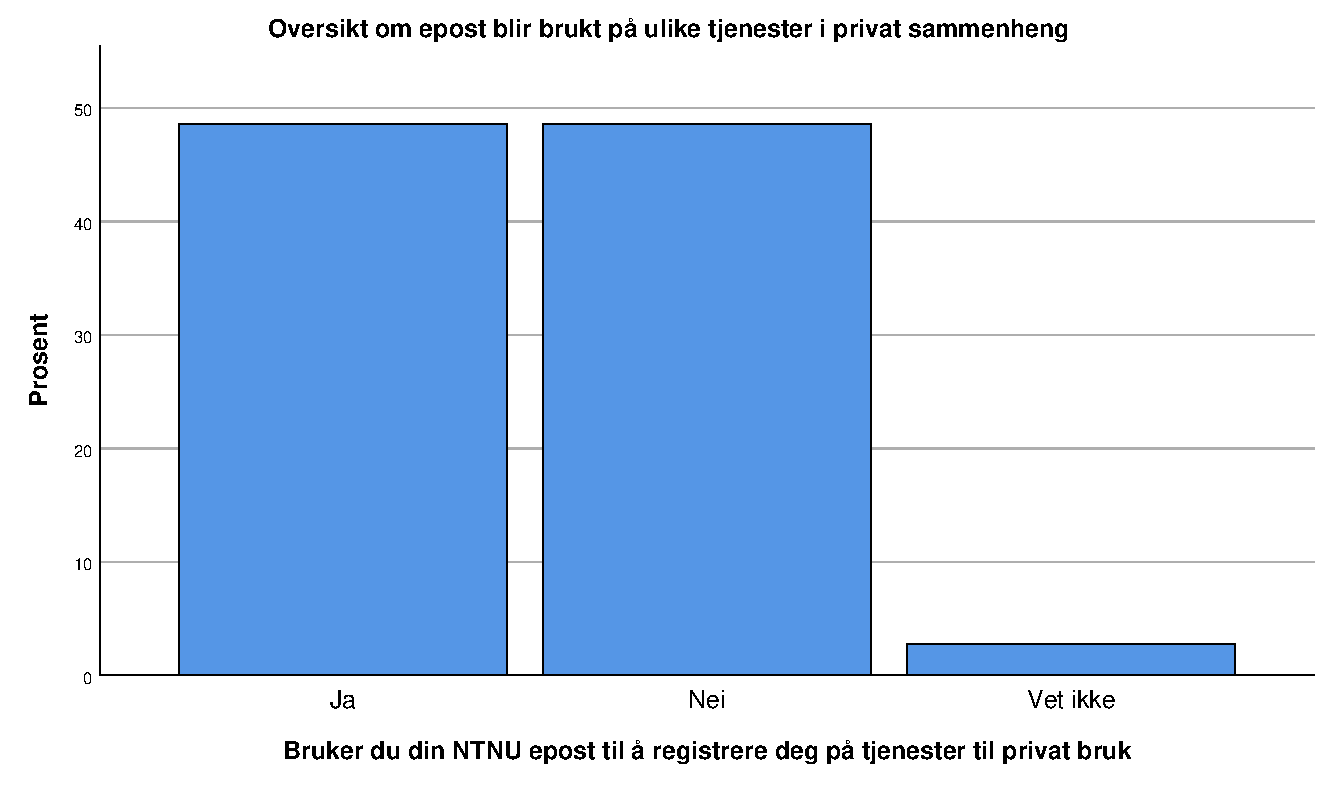
\includegraphics[scale=0.5]{case_2/bilder/spss/epost_privat.pdf}
    \caption[E-post til private tjenester]{Viser hvor mange som bruker NTNU e-post til private tjenester}
    \label{fig:case2-epost-privat}
\end{figure}
Hypotesen vår var korrekt, litt under halvparten bruker NTNU e-posten til privat bruk. Selv om det er under halvparten som bruker NTNU e-posten til privat bruk, så er dette noe som burde unngås. 

Over 50\% av respondentene bruker NTNU passordet på flere tjenester som vist i figuren under. 
\begin{figure}[H]
    \centering
    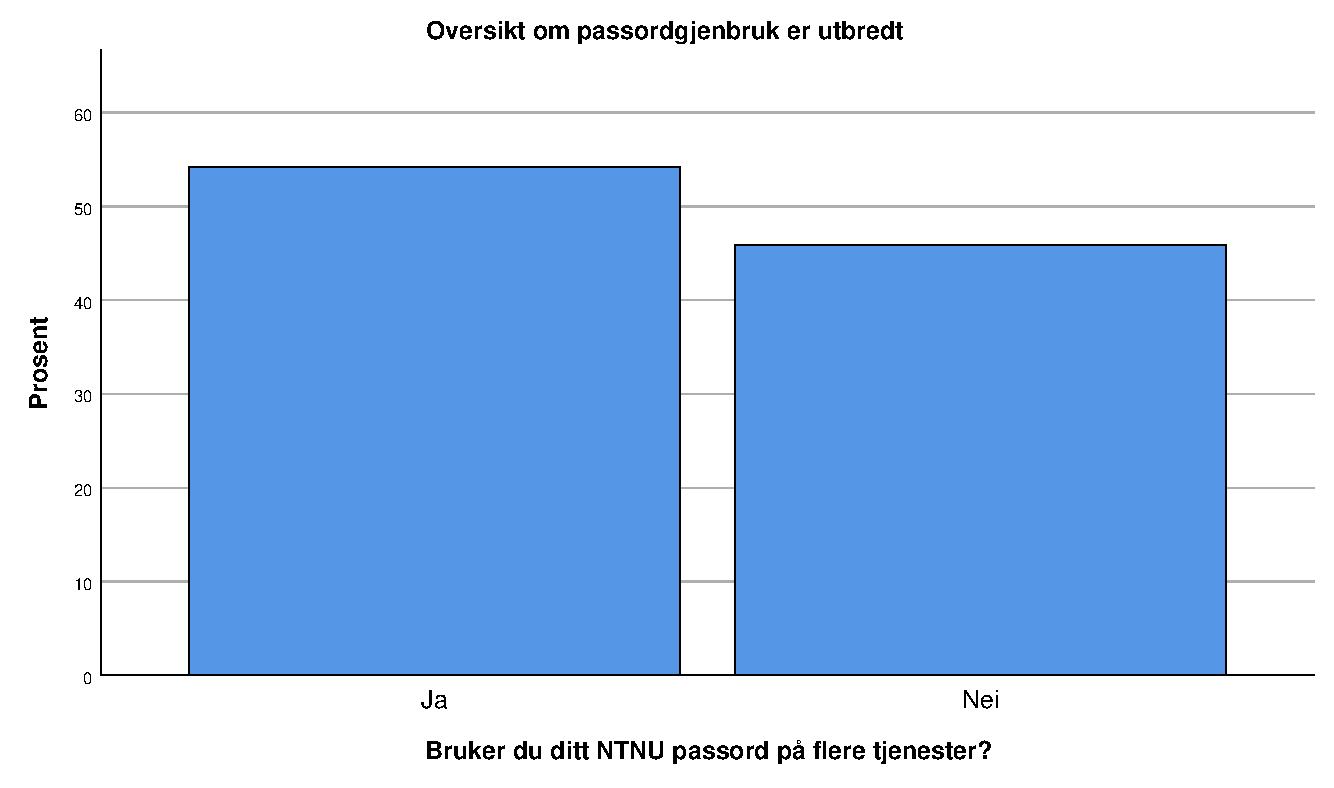
\includegraphics[scale=0.5]{case_2/bilder/spss/passordgjenbruk.pdf}
    \caption[Frekvens av passordgjenbruk]{Oversikt over gjenbruk av NTNU passord}
    \label{fig:case2-passordgjenbruk}
\end{figure}
Hypotesen vår her var korrekt, over halvparten bruker samme NTNU passord på flere tjenester. Dette var også en av hovedhypotesene til caset. 

Over 80\% av respondentene svarte at de ikke brukte regler til å generere passord. Det er mulig for feiltolkning av spørsmålet, i og med at regler kan bety to forskjellige ting. Det kan bety regle, i form av ``Lisa-gikk-til-NTNU'' for NTNU-passord, eller så kan man tolke det som en regel. 
\begin{figure}[H]
    \centering
    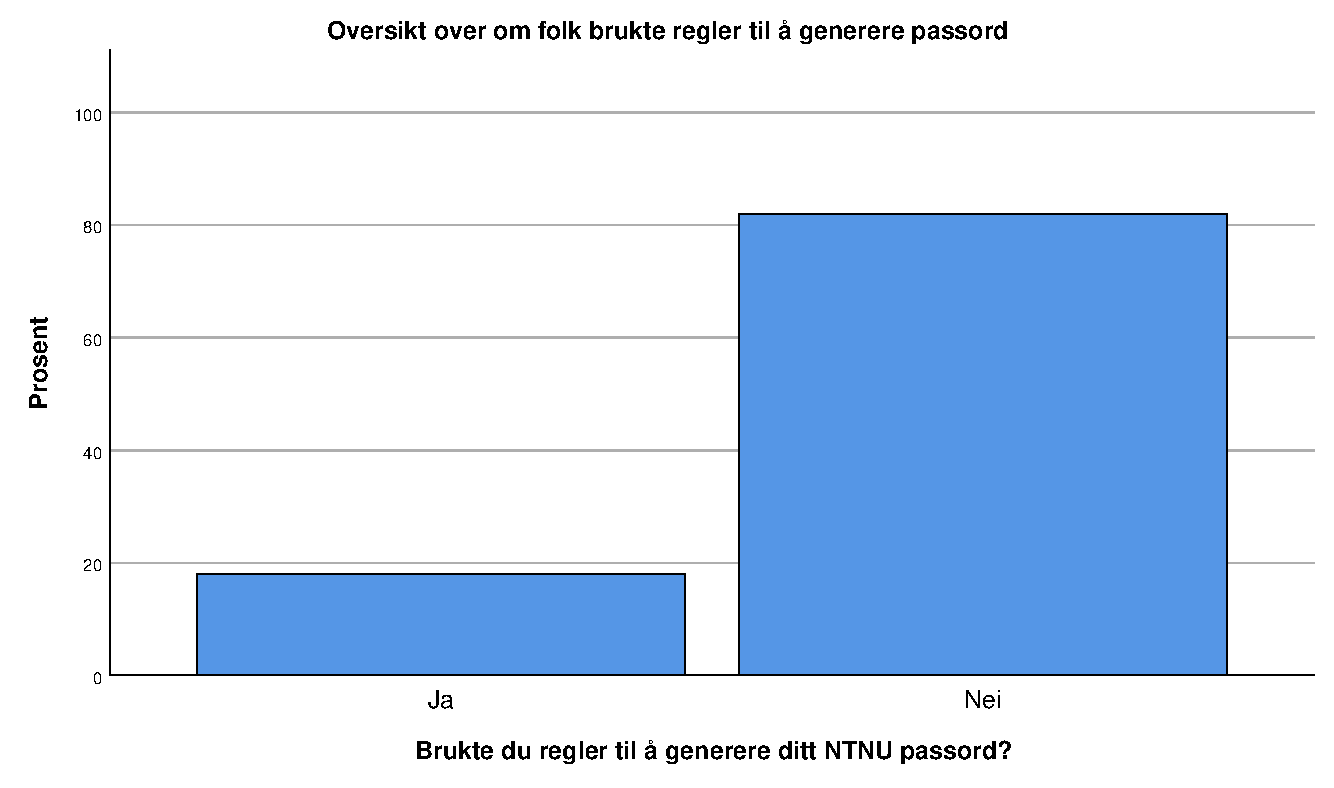
\includegraphics[scale=0.5]{case_2/bilder/spss/regler_passord.pdf}
    \caption[Bruk av passordregler]{Viser hvor mange som bruker passordregler}
    \label{fig:case2-passordregler}
\end{figure}
Vi kan derfor ikke si noe med sikkerhet om hypotesen vår ble bekreftet eller avkreftet.

Over 80\% av respondentene har passord som er mellom 8-11 tegn. Resterende fordelte seg likt utover de andre valgene. 
\begin{figure}[H]
    \centering
    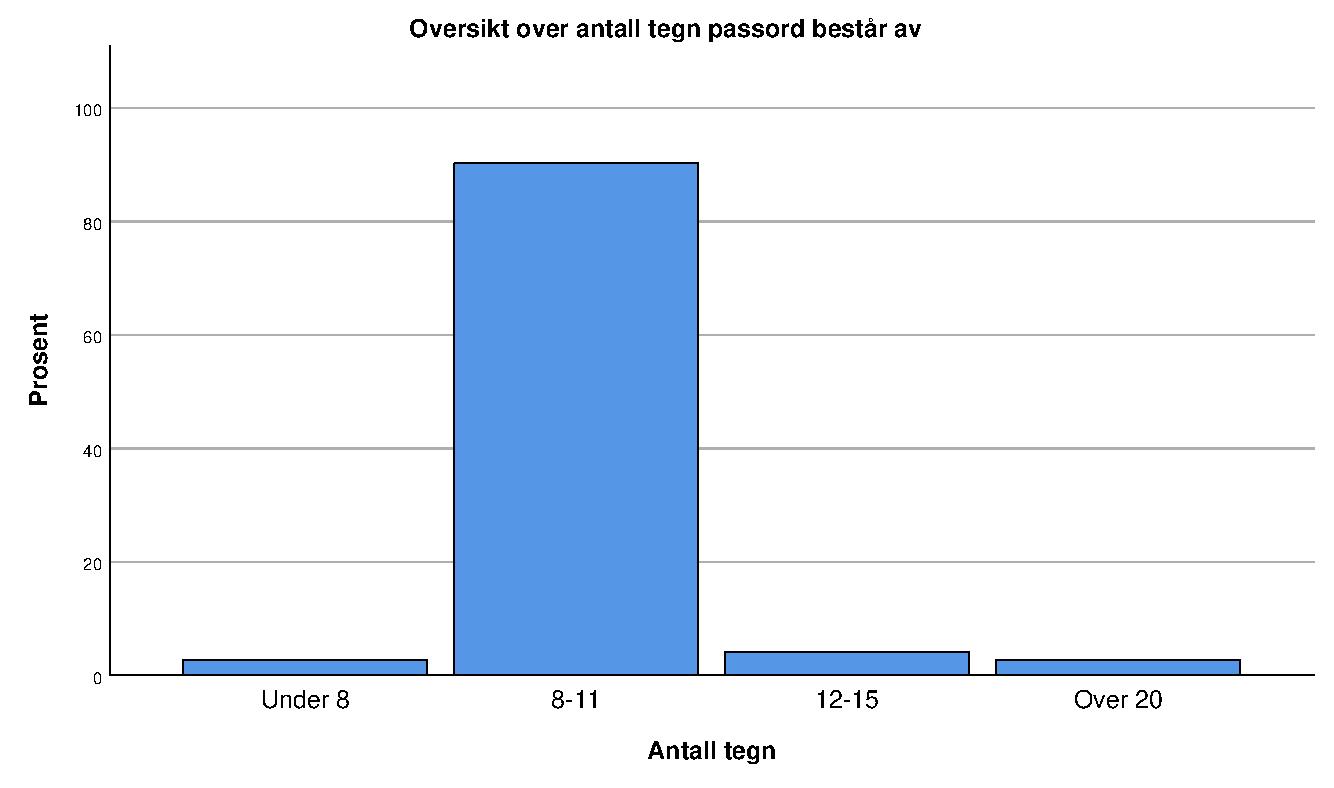
\includegraphics[scale=0.5]{case_2/bilder/spss/antall_tegn.pdf}
    \caption[Antall tegn i passord]{Antall tegn på passord}
    \label{fig:case2-antalltegn}
\end{figure}
Hypotesen vår var korrekt, de fleste bruker passord som er under 12 tegn. Det er mulig vi burde ha splittet opp intervallene ytterligere jo mindre antall tegn det var snakk om. 

Figur \ref{fig:case2-bytter-passord} viser statistikken over hvor ofte respondentene bytter passord. Over 50\% sier at de bytter passord sjeldnere enn hvert andre år, over 20\% sier at de bytter hvert andre år, rett under 20\% sier at de bytter hvert år og resten sier at de bytter hver sjette måned. 
\begin{figure}[H]
    \centering
    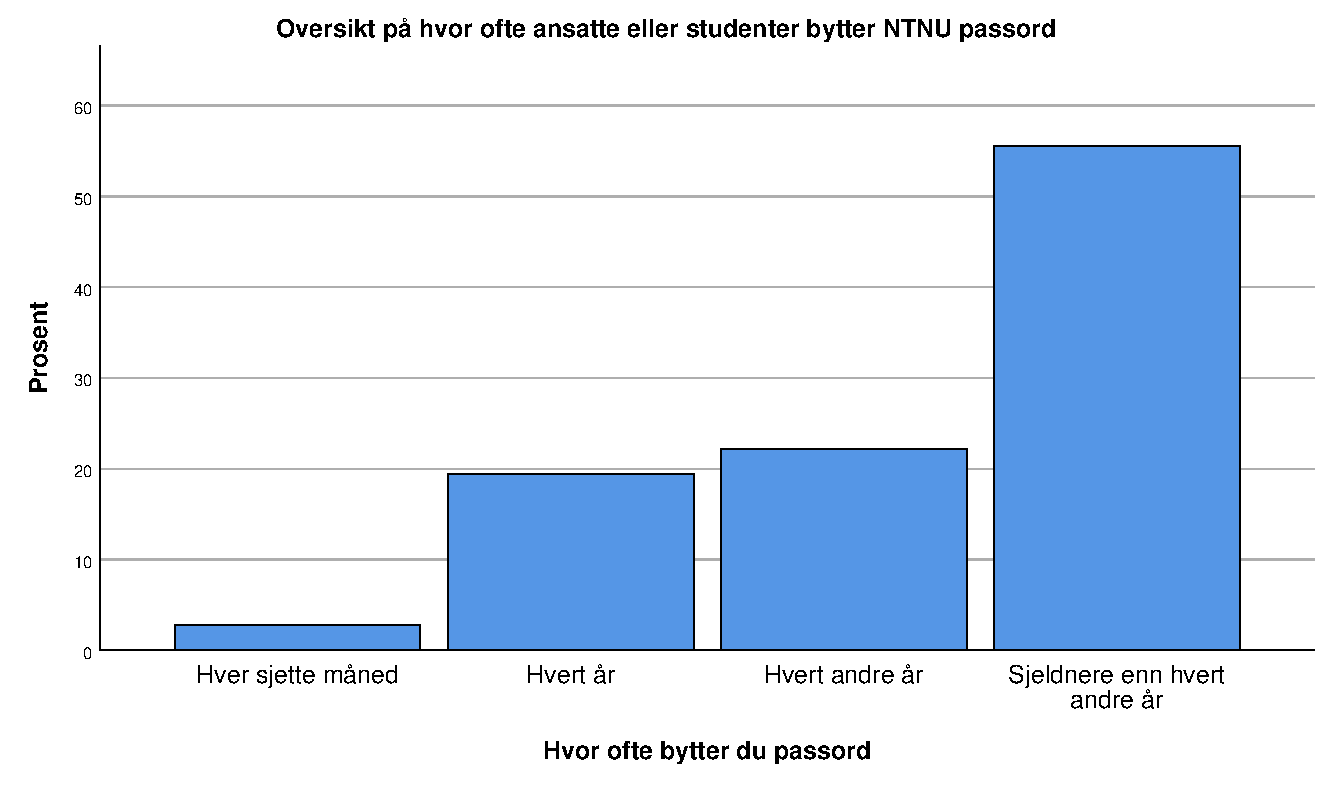
\includegraphics[scale=0.5]{case_2/bilder/spss/bytter_passord.pdf}
    \caption[Hvor ofte de bytter passord]{Viser hvor ofte de bytter passord}
    \label{fig:case2-bytter-passord}
\end{figure}
Hypotesen var korrekt, flertallet av respondentene bytter passord sjeldnere enn hvert andre år. I henhold til en innsida-side som beskriver hvordan en skal håndtere slike data så skal passord byttes hver sjette måned og tvungen passordbytte hvert år. Dette viser at respondentene ikke kjent med disse retningslinjene. 

I figur \ref{fig:case2-passordsikkerhet} ser vi antallet som sier at de har fått opplæring i passordsikkerhet fra NTNU. Ut fra tabellen ser vi at under 80\% av respondentene sier at de ikke har fått opplæring i passordsikkerhet. 15\% sier at de ikke vet om de har fått opplæring og resten sier at de har fått det. 
\begin{figure}[H]
    \centering
    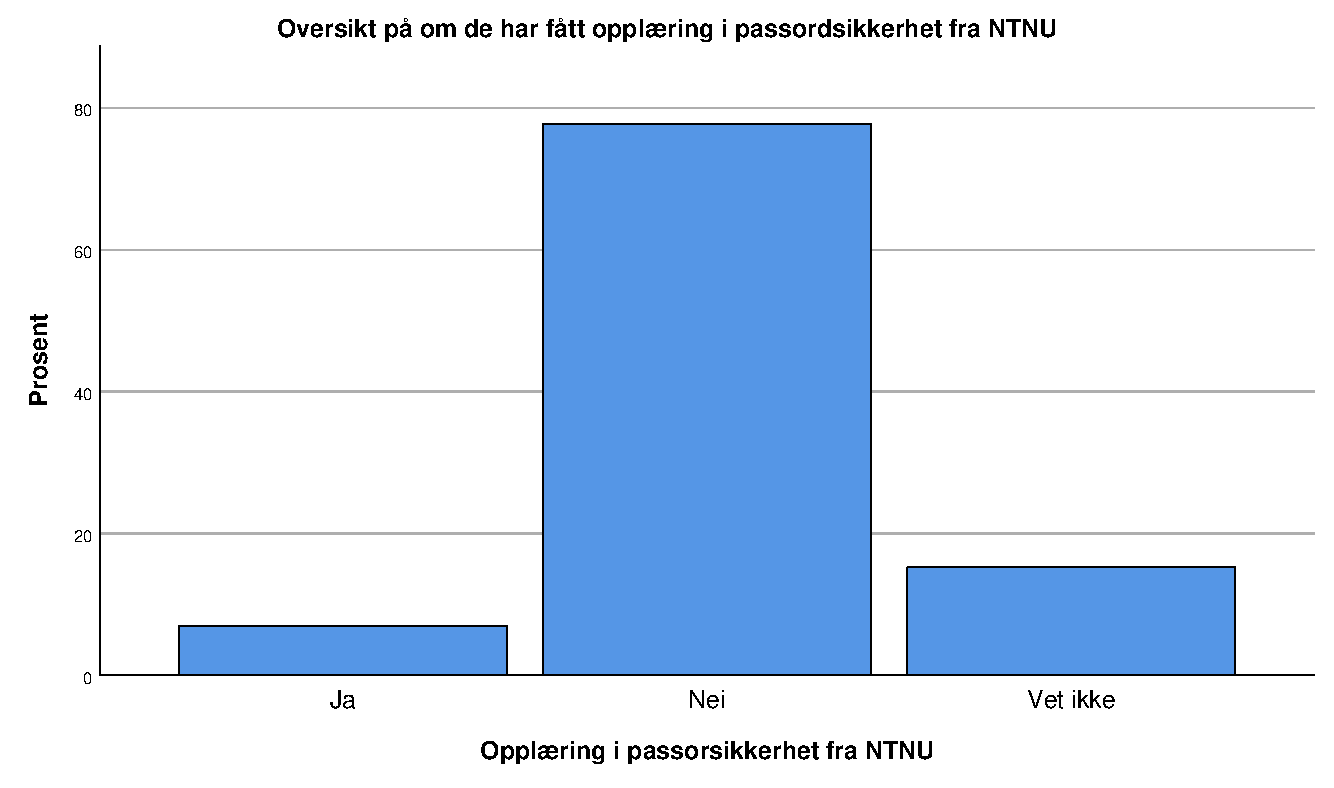
\includegraphics[scale=0.5]{case_2/bilder/spss/opplaring_passordsikk_NTNU.pdf}
    \caption[Opplæring i passordsikkerhet]{Viser hvor mange som har fått opplæring i passordsikkerhet}
    \label{fig:case2-passordsikkerhet}
\end{figure}

\subsection{Phishing}
Over 70\% av respondentene sa at de har oppdaget phishing e-post en eller flere ganger på sin NTNU e-post, og rett under 20\% som ikke har oppdaget phishing e-post. Resten av respondentene svarte at de ikke vet. Dette vises i figur \ref{fig:case2-oppdaget-phishing} under.
\begin{figure}[H]
    \centering
    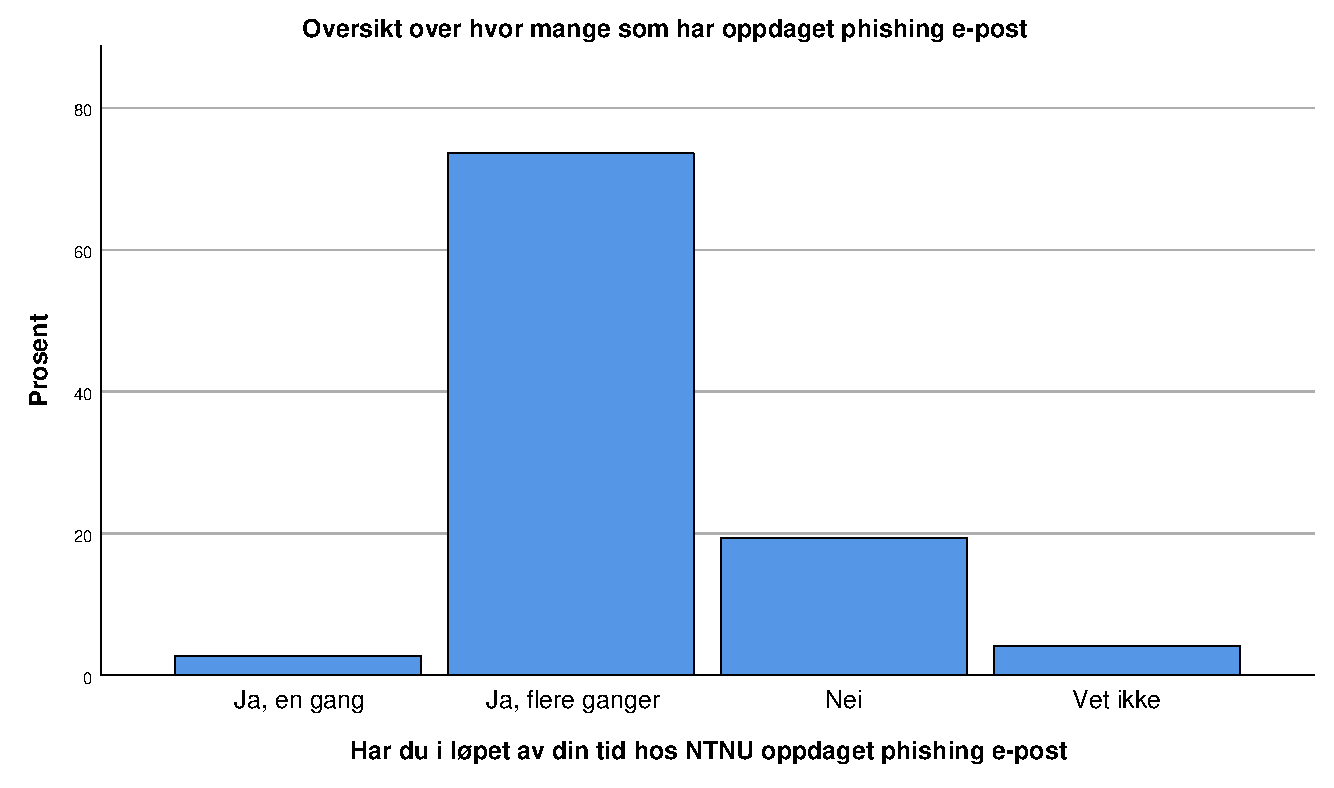
\includegraphics[scale=0.5]{case_2/bilder/spss/oppdaget_phish.pdf}
    \caption[Oppdaget phishing]{Viser hvor mange som har oppdaget phishing e-post}
    \label{fig:case2-oppdaget-phishing}
\end{figure}

Over 70\% av respondentene sier at de ikke har blitt lurt av phishing e-post, og under 20\% sier at de har blitt lurt. Som vist i tabellen under. 
\begin{figure}[H]
    \centering
    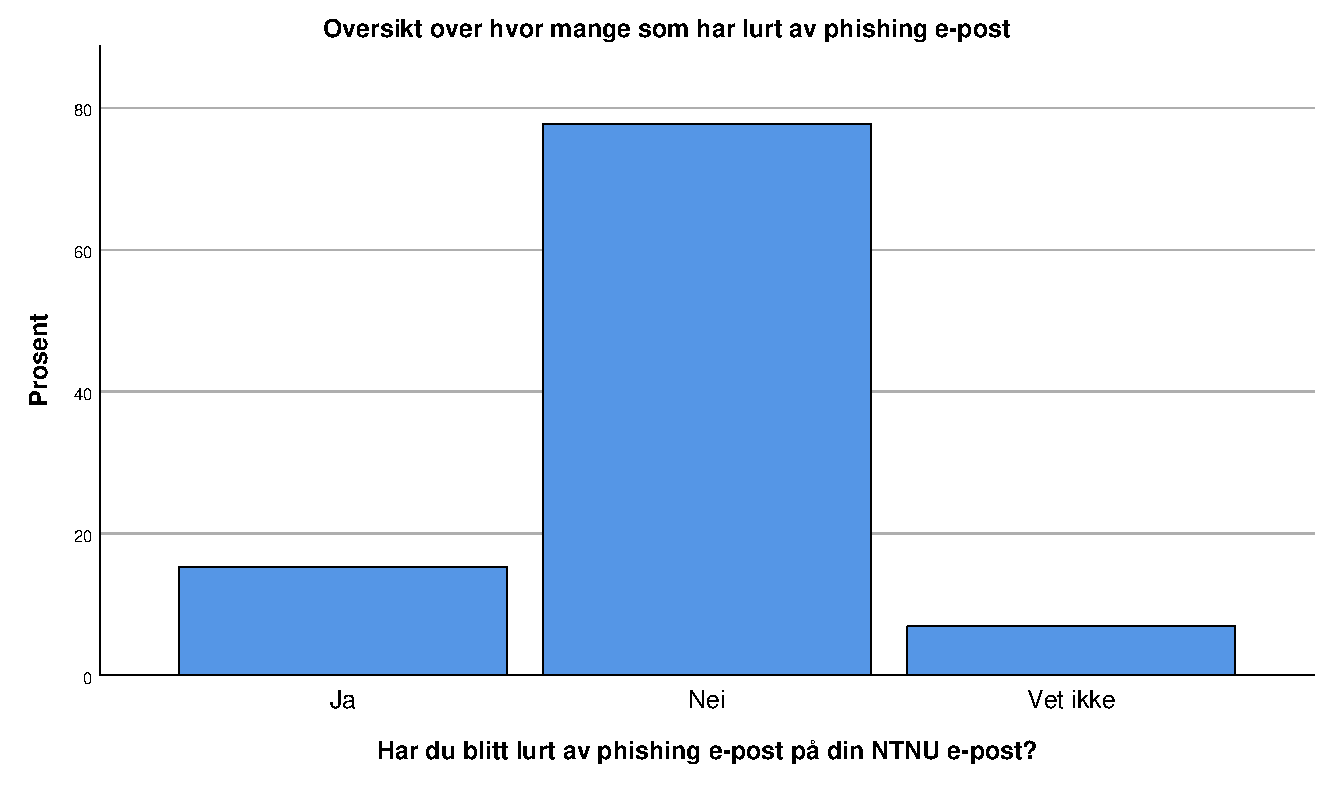
\includegraphics[scale=0.5]{case_2/bilder/spss/lurt_phish.pdf}
    \caption[Lurt av phishing]{Viser hvor mange som sier de har blitt lurt av phishing}
    \label{fig:lurt-av-phishing}
\end{figure}

\subsection{Statistisk analyse}
I denne delen bruker vi statistiske analyseverktøy for å finne relasjoner. De mindre relevante analysene er plassert i vedlegg \ref{vedlegg:statanalys}. Som en generell regel for utføring av analysen har vi valgt et signifikansnivå på: \[\alpha \leq 0,05\]

\subsubsection{ANOVA på alder mot bevissthet og kjennskap}
Denne testen sjekker om det er signifikans mellom alder på respondenten, og hvor bevisste de er på sikkerhet og hvor godt de kjenner til de ulike retningslinjene og reglementene. Alle spørsmålene er besvart på en skala fra 1 til 6, der 1 er lite bevisst eller kjent, og 6 er svært bevisst eller kjent. I tabellen under beskrives svarene til datasettet som er analysert. 
\begin{figure}[H]
    \centering
    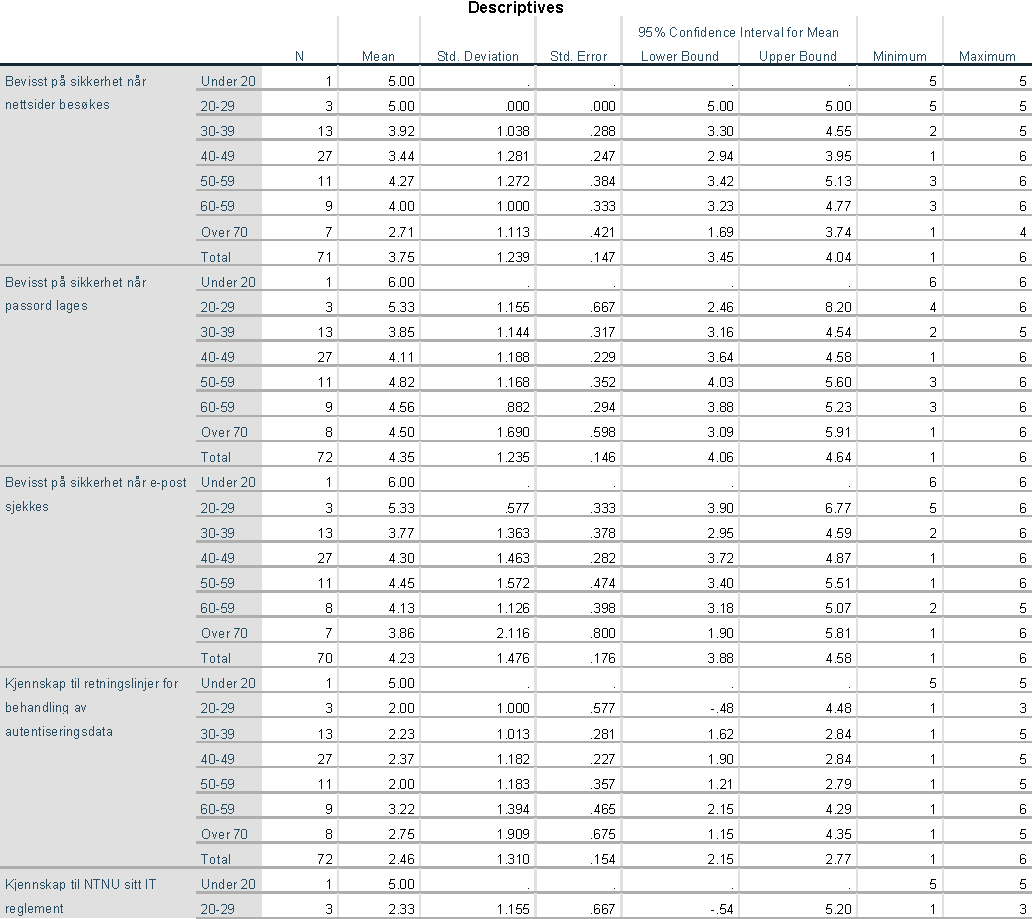
\includegraphics[scale=0.7]{case_2/bilder/spss/anova_ttest/alder_bevissthetogkjennskap_descriptive_1.pdf}
    \caption[Descriptive av alder mot bevissthet på sikkerhet og kjennskap til dokumenter del 1]{Descriptive av alder mot bevissthet på sikkerhet og kjennskap til retningslinjer, del 1}
    \label{fig:alder-bevissthetogkjennskap-descriptive-1}
\end{figure}

\begin{figure}[H]
    \centering
    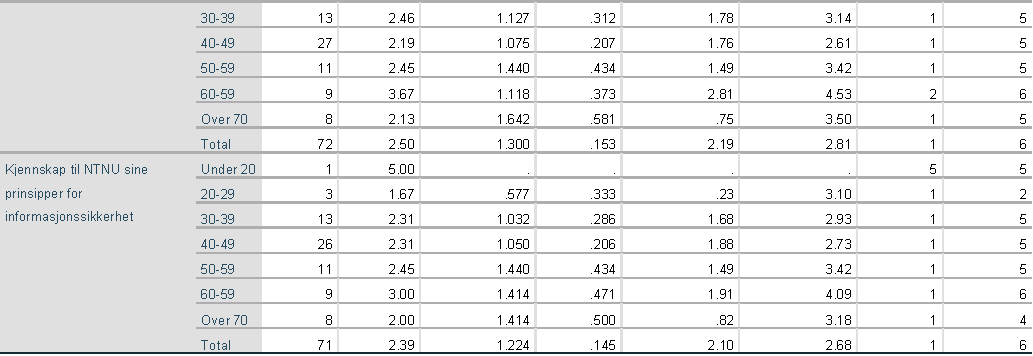
\includegraphics[scale=0.7]{case_2/bilder/spss/anova_ttest/alder_bevissthetogkjennskap_descriptive_2.pdf}
    \caption[Descriptive av alder mot bevissthet på sikkerhet og kjennskap til dokumenter del 1]{Descriptive av alder mot bevissthet på sikkerhet og kjennskap til retningslinjer, del 2}
    \label{fig:alder-bevissthetogkjennskap-descriptive-2}
\end{figure}

Fra dataene over kan vi se at generelt sett går bevisstheten på sikkerhet og kjennskapen til retningslinjene ned etterhvert som respondentene blir eldre. Dette gjelder spesielt for bevissthet på sikkerhet når nettsider besøkes og kjennskap til IT-reglementet. 

\begin{figure}[H]
    \centering
    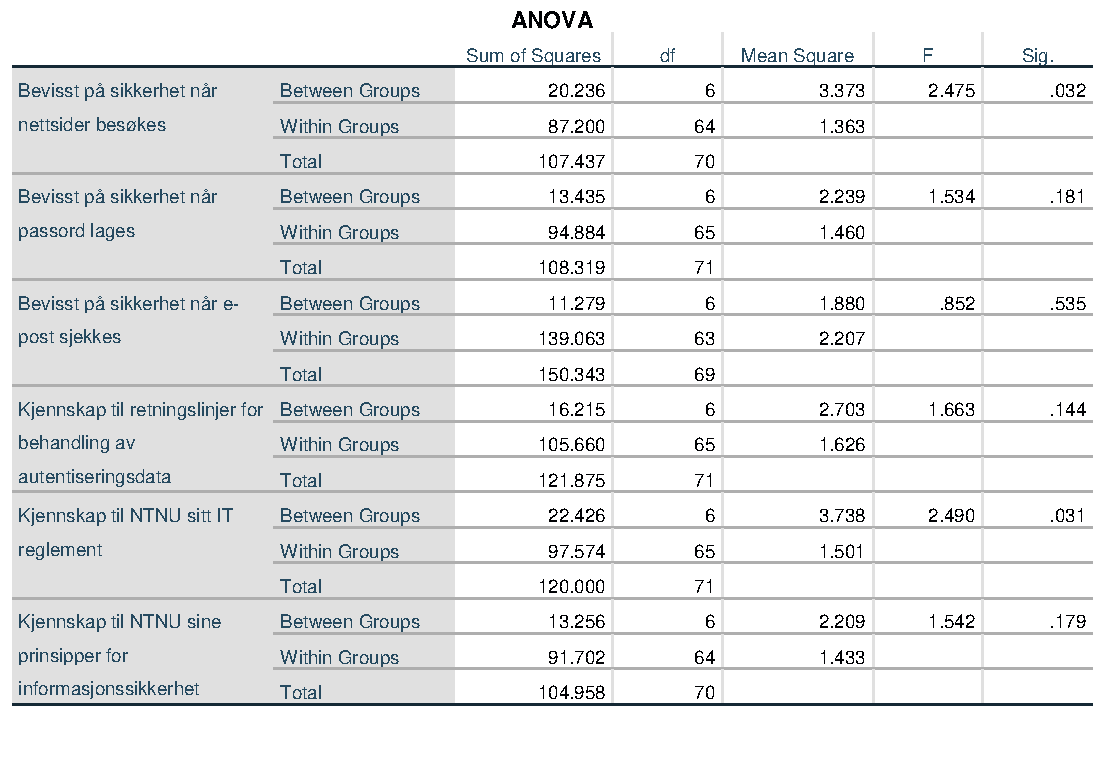
\includegraphics[scale=0.7]{case_2/bilder/spss/anova_ttest/alder_bevissthetogkjennskap_anova.pdf}
    \caption[ANOVA av alder mot bevissthet på sikkerhet og kjennskap til retningslinjer]{ANOVA av alder mot bevissthet på sikkerhet og kjennskap til dokumenter}
    \label{fig:alder-bevissthetogkjennskap-ANOVA}
\end{figure}

I tabellen over ser vi at når det kommer til alder basert på bevissthet på sikkerhet når nettsider besøkes er dette signifikant siden \(\alpha = 0,032\). Dette betyr at vi kan konkludere med at jo eldre folk blir, jo mindre bevisste er de på sikkerhet når de besøker nettsider. Dette gjelder også for kjennskap til NTNU sitt IT-reglement, der signifikansen er på \(\alpha = 0,031\). 

En post-hoc test kunne ikke kjøres her fordi en av kategoriene bare hadde ett svar. 

\subsubsection{ANOVA på år ved NTNU mot passord-, e-post- og andre brukervaner}
Denne testen sjekker om det er signifikans mellom antall år respondenten har vært hos NTNU, og om de bruker NTNU e-posten sin på andre tjenester, om de har blitt lurt av phishing og om de benytter sitt NTNU passord på flere tjenester. I tabellen under beskrives svarene til datasettet vi skal analysere.
\begin{figure}[H]
    \centering
    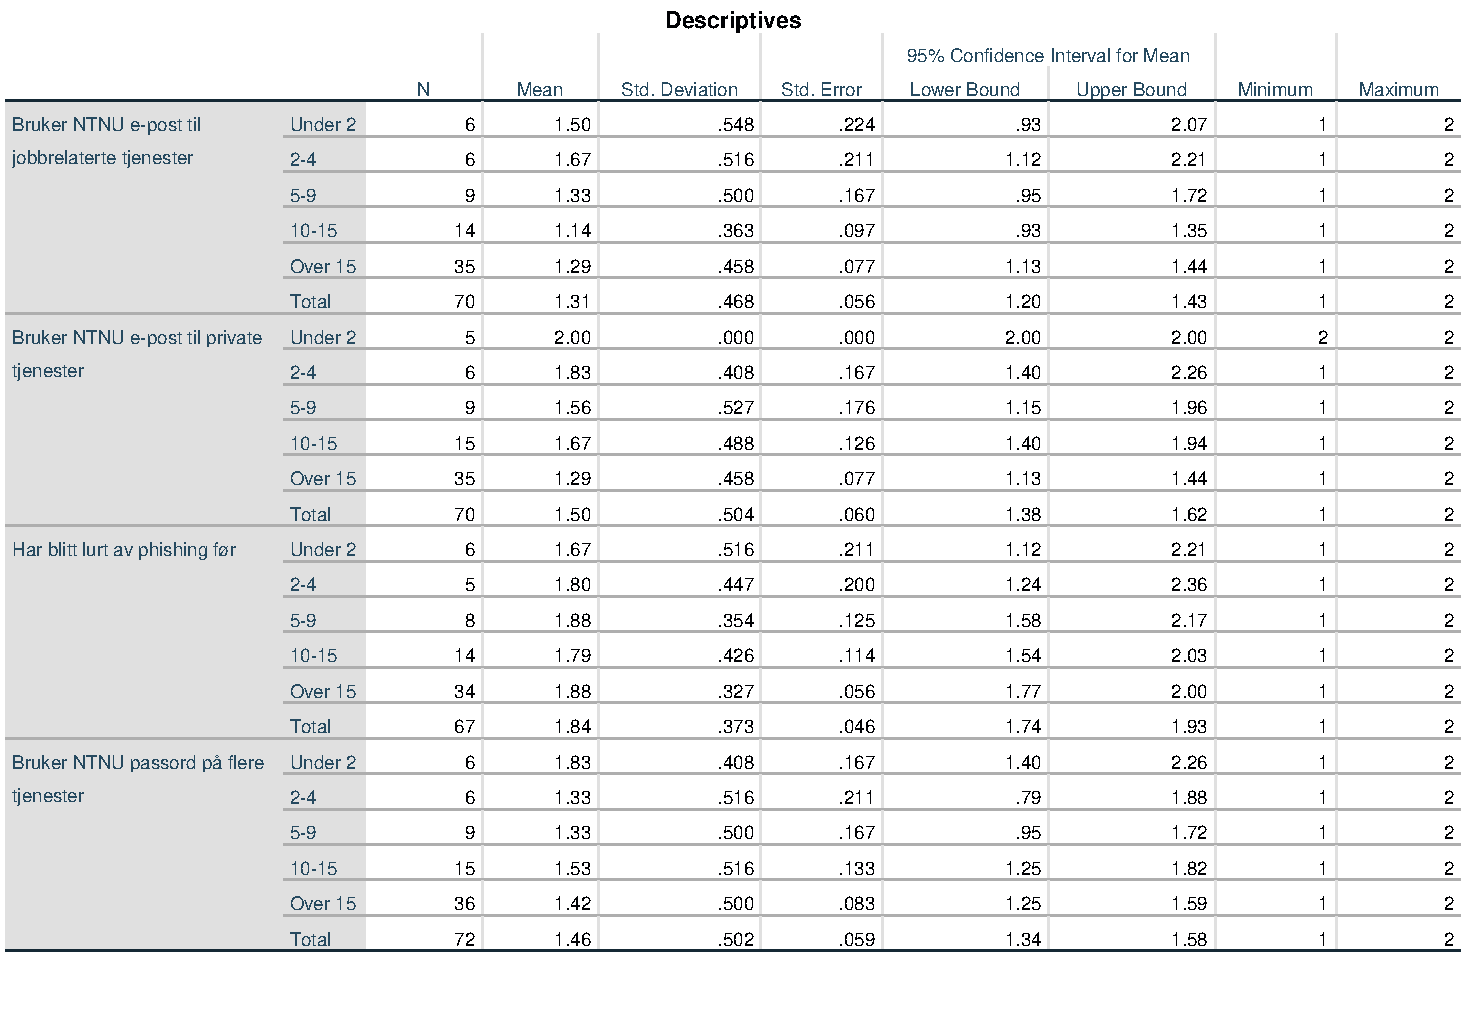
\includegraphics[scale=0.5]{case_2/bilder/spss/anova_ttest/ansiennitet_diverse_descriptive.pdf}
    \caption[Descriptive av år ved NTNU mot passord-, e-post- og andre brukervaner]{Descriptive av år ved NTNU mot passord-, e-post- og andre brukervaner}
    \label{fig:ansiennitet-diverse-descriptive}
\end{figure}

\begin{figure}[H]
    \centering
    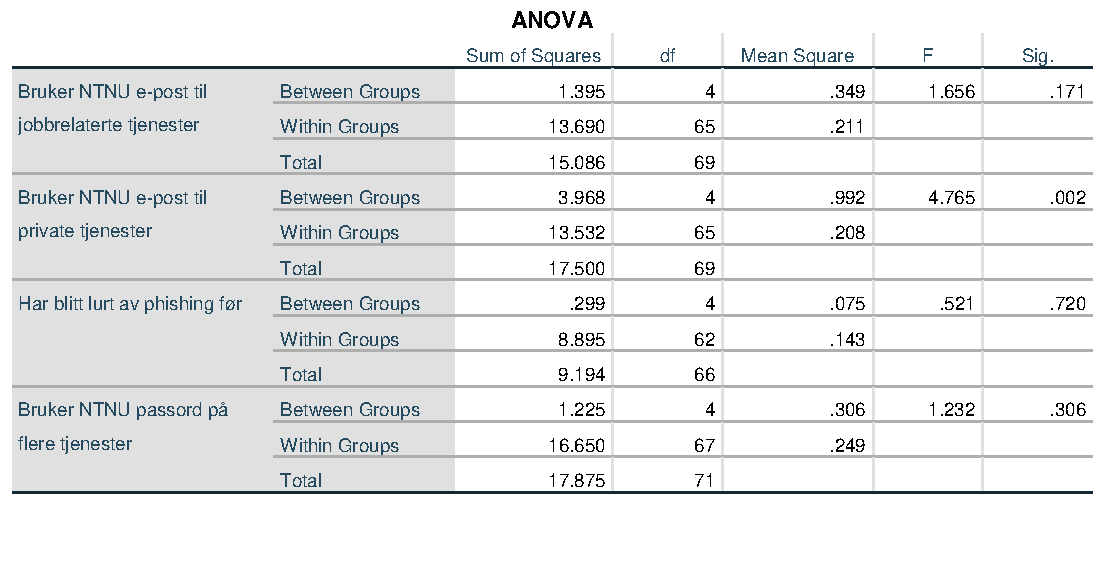
\includegraphics[scale=0.7]{case_2/bilder/spss/anova_ttest/ansiennitet_diverse_anova.pdf}
    \caption[ANOVA av år ved NTNU mot passord-, e-post- og andre brukervaner]{ANOVA av år ved NTNU mot passord-, e-post- og andre brukervaner}
    \label{fig:ansiennitet-diverse-ANOVA}
\end{figure}

Siden det er signifikans på de som bruker NTNU e-post til private tjenester (\(\alpha \leq 0,05\)), ble en post-hoc test kjørt for å se om det var noen ytterligere signifikans mellom gruppene. Grunnet plassbesparelse er bare de variablene som inkluderte signifikans tatt med i rapporten. 

\begin{figure}[H]
    \centering
    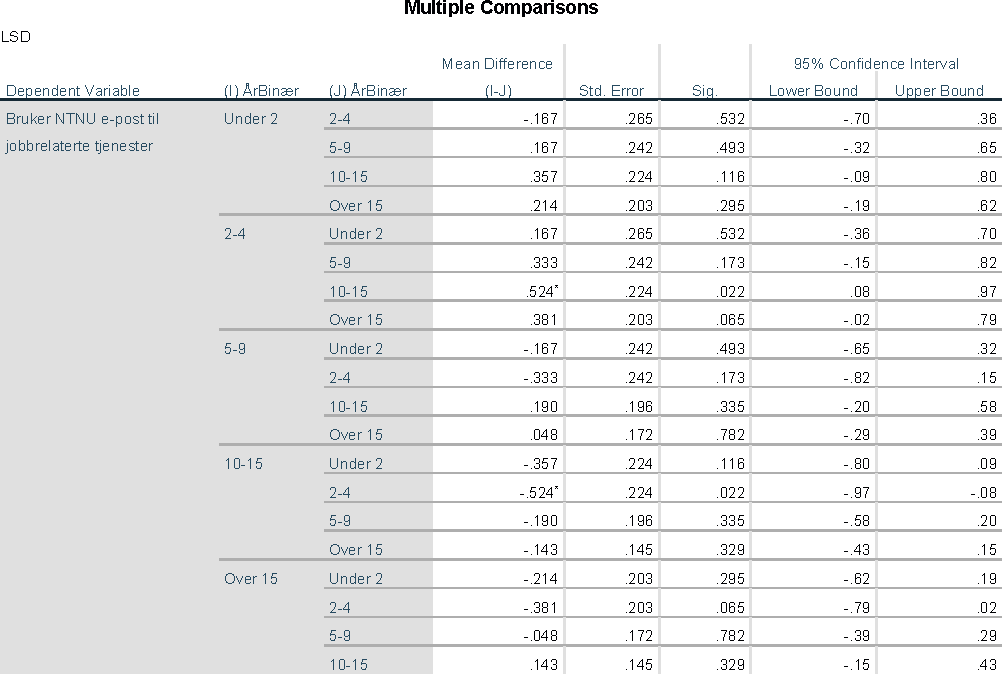
\includegraphics[scale=0.7]{case_2/bilder/spss/anova_ttest/ansiennitet_diverse_posthoc_1.pdf}
    \caption[Post-hoc av år ved NTNU mot passord-, e-post- og andre brukervaner del 1]{Post-hoc av år ved NTNU mot passord-, e-post- og andre brukervaner, del 1}
    \label{fig:alder-bevissthetogkjennskap-posthoc-1}
\end{figure}

\begin{figure}[H]
    \centering
    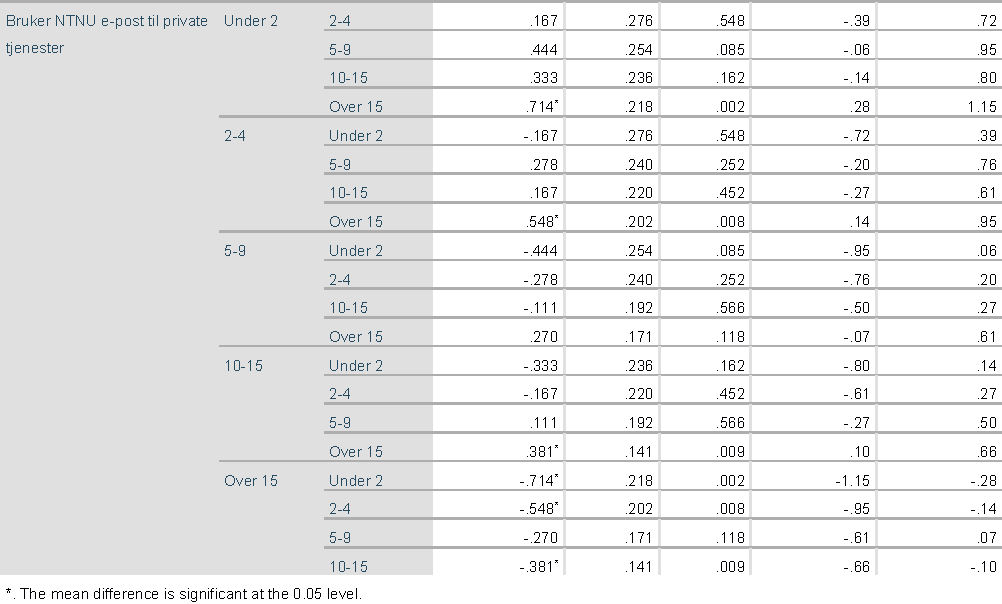
\includegraphics[scale=0.7]{case_2/bilder/spss/anova_ttest/ansiennitet_diverse_posthoc_2.pdf}
    \caption[Post-hoc av år ved NTNU mot passord-, e-post- og andre brukervaner del 2]{Post-hoc av år ved NTNU mot passord-, e-post- og andre brukervaner, del 2}
    \label{fig:alder-bevissthetogkjennskap-posthoc-2}
\end{figure}

I post-hoc testen i figur \ref{fig:alder-bevissthetogkjennskap-posthoc-1} og \ref{fig:alder-bevissthetogkjennskap-posthoc-2} ser vi at når det kommer til jobbrelaterte tjenester er forskjellen signifikant mellom de som har vært ved NTNU i 2-4 år og 10-15 år. Når det kommer til private tjenester er forskjellen signifikant mellom under 2 år og over 15, 2-4 år og over 15, og mellom 10-15 år og over 15. Vi ser at det er en relasjon mellom hvor mange år ved NTNU de og om de bruker NTNU e-post på andre tjenester. Jo lenger de er der, jo mer sannsynlig er det at de bruker e-posten på flere tjenester. 

\subsubsection{ANOVA på alder mot passord-, e-post- og andre brukervaner}
Siden det ble funnet signifikans på antall år ved NTNU og bruk av NTNU e-post på private tjenester, kunne det være sannsynlig at dette også korrelerte med alder. Det er logisk å tro at jo lenger tid en har tilbringet ved NTNU, jo eldre er personen. Derfor ble det kjørt en korrelasjonstest på alder og antall år ved NTNU for å teste dette. I tabellen under kan vi se at det er en sterk positiv korrelasjon (\(\alpha \le 0,01\)) mellom alder og tid ved NTNU.

\begin{figure}[H]
    \centering
    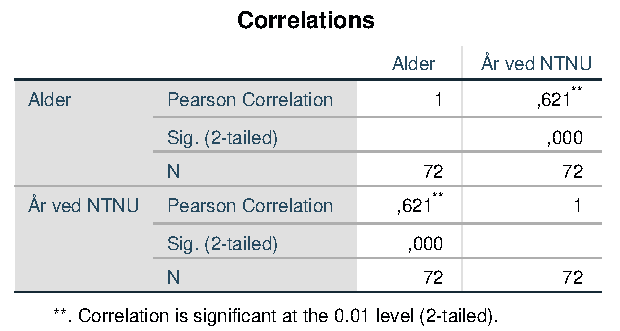
\includegraphics[scale=1]{case_2/bilder/spss/anova_ttest/alder_aarvedNTNU_korrelasjon.pdf}
    \caption[Korrelasjon mellom alder og antall år ved NTNU]{Korrelasjon mellom alder og antall år ved NTNU}
    \label{fig:alder-aarvedNTNU-korrelasjon}
\end{figure}

Basert på resultatene er det grunnlag for å tro at siden jo eldre respondenten som har fått sin konto kompromittert er, jo mer sannsynlig er det at personen har benyttet e-posten på private tjenester, basert på resultatene i figur \ref{fig:ansiennitet-diverse-ANOVA} i forrige seksjon.

\subsection{Independent sample t-test på de som har delt passord mot hvor ofte de bytter passord}
Selv om det bare er åtte personer som har sagt at de har delt sitt NTNU passord er dette åtte personer for mye. I IT-reglementet står det at dersom du har mistanke om at noen kan passordet, skal du bytte det med en gang \cite{ITReg}. Derfor var det relevant å se hvor ofte de som har delt passordet sitt bytter passord. Variabelen ``ByttePassordBinær'' går fra 1-4 der 1 er bytte av passord hver sjette måned og 4 er hvert andre år. 

\begin{figure}[H]
    \centering
    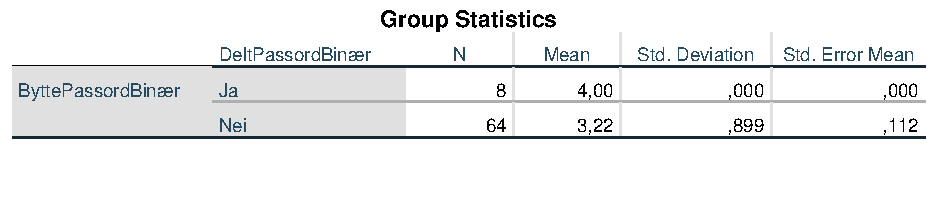
\includegraphics[scale=0.7]{case_2/bilder/spss/anova_ttest/deltpassord_byttepassord_groupstats.pdf}
    \caption[Group statistics av de som har delt passord mot hvor ofte de bytter]{Group statistics av de som har delt passord mot hvor ofte de bytter}
    \label{fig:deltpassord-byttepassord-groupstats}
\end{figure}

Statistikken i figur \ref{fig:deltpassord-byttepassord-groupstats} over viser at alle de som har delt passordet sitt, bytter passord sjeldnere enn hvert andre år. Dette er bekymringsfullt i og med at passordene er kjent av andre over lengre tid. I figur \ref{fig:deltpassord-byttepassord-ttest} sjekker vi om disse tallene er signifikante.

\begin{figure}[H]
    \centering
    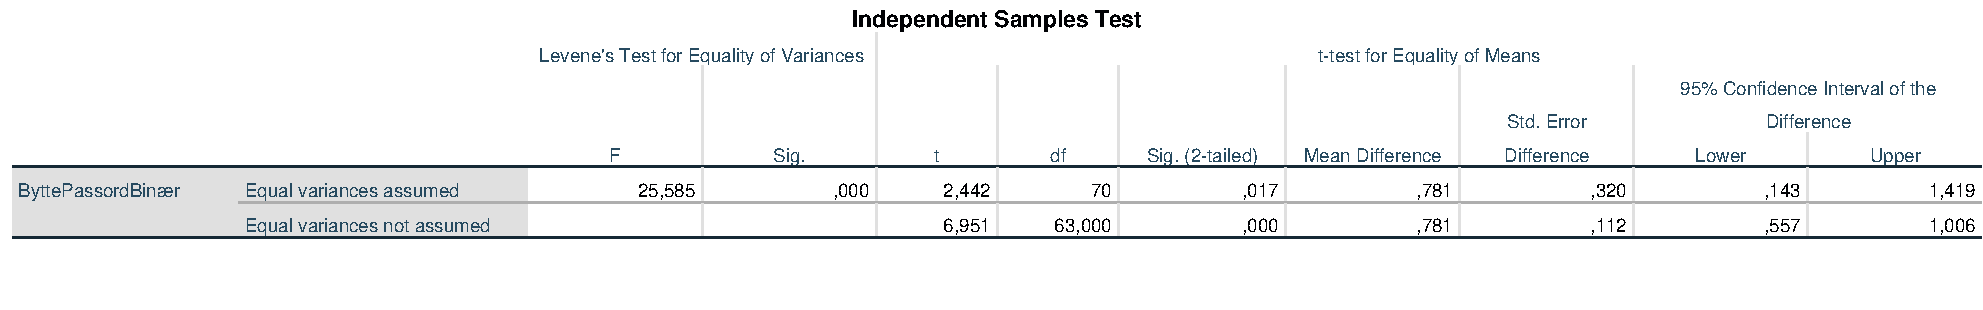
\includegraphics[scale=0.4]{case_2/bilder/spss/anova_ttest/deltpassord_byttepassord_ttest.pdf}
    \caption[Independent t-test av de som har delt passord mot hvor ofte de bytter]{Independent t-test av de som har delt passord mot hvor ofte de bytter}
    \label{fig:deltpassord-byttepassord-ttest}
\end{figure}

Vi kan se at \(\alpha = 0,017\), som betyr at resultatet er statistisk signifikant. 


\section{Rotårsaksidentifisering}

\subsection{Årsak-virkningsdiagram}
Innledningsvis ble problemet beskrevet som rotårsaken til kompromitterte kontoer ved NTNU. Hovedkategoriene som ble undersøkt for å finne svar på dette var gjenbruk av innloggingskredentialier tilhørende NTNU, IT-reglementet og andre styringsdokumenter, passordvaner, phishing og oversikt over situasjonen. Både hovedkategoriene og årsakene under disse er i hovedsak basert på dataanalysen, mens noe er basert på kreativ idémyldring. 

\begin{figure}[H]
    \centering
    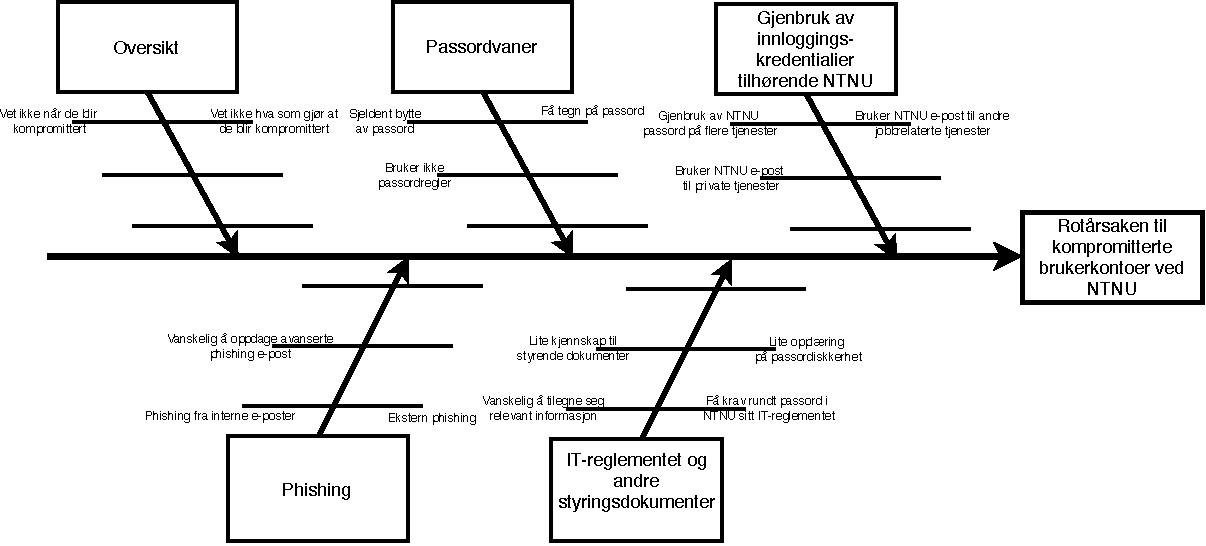
\includegraphics[scale=0.65]{case_2/bilder/fiskebein.pdf}
    \label{fig:fiskebein-case2}
    \caption[Fiskebeindiagram for kompromitterte kontoer]{Fiskebeindiagram over hovedkategorier og årsaker til kompromitterte kontoer}
\end{figure}

Vi har kommet frem til at rotårsaken til kompromitterte kontoer er sammensatt av flere faktorer. Et passord på mellom åtte til elleve tegn i seg selv er ikke nok for at kontoen skal bli kompromittert, men sammen med at de bytter sjeldnere enn hvert andre år gjør at dette blir et problem. I tillegg til dette bruker flertallet NTNU e-posten til andre tjenester, enten til jobbrelatert eller til privat bruk. De bruker også samme NTNU passord på flere tjenester. Dette er noe en burde unngå til enhver tid, og er noe av det vi anser å være blant det mest kritiske. 

Respondentene hadde også liten kjennskap til IT-reglementet og andre styringsdokumenter. De svarte også at de har fått lite opplæring på passordsikkerhet. Vi har lest gjennom IT-reglementet og andre styringsdokumenter, og har kommet frem til at IT-reglementet har for få krav til passord. Det var vanskelig å tilegne seg all informasjon på de forskjellige styringsdokumentene da IT-reglementet ikke henviste til noen av retningslinjene. I retningslinjer for behandling av brukernavn, passord og andre autentiseringsdata \cite{RetnBPA} står det at passordet skal byttes hver 12 måned. Denne retningslinjen er ikke nevnt i IT-reglementet at du skal gjøre deg bekjent med. 

Sammenlagt så viste det oss at respondentene hadde dårlige passordvaner, gjenbruk av innloggingskredentialier tilhørende NTNU og lite kunnskap til IT-reglementet og andre styrende dokumenter. Phishing er også en relevant årsak til kompromitterte kontoer. Phishing e-poster har blitt såpass sofistikerte at det er vanskelig å skille mellom falske og legimite e-poster. \cite{SophPhish}. Rotårsakene er derfor som følger: 

\begin{itemize}
    \item Mistet kontodetaljer av phishing
    \item E-post og passordgjenbruk på andre tjenester
    \item Liten kjennskap til IT-reglement og andre styrende dokumenter
    \item Dårlige passordvaner
\end{itemize}

\subsection{5 Whys}
Det ble fremhevet fem årsaker som skulle analyseres. Fire av disse kom fra fiskebeindiagrammet over, og en fra idémyldring. Tabellene under viser resultatene fra gjennomføringen. 

\begin{table} [H]
    \centering
    \begin{tabular}{ | m{5em} | m{30em} | }
        \hline
            \cellcolor{yellow} Årsak: & \cellcolor{yellow} Mistet kontodetaljer av phishing                \\
        \hline
            Why? & Fordi e-posten kom fra en intern e-postadresse                                   \\
        \hline
            Why? & Fordi kontoen var blitt kompomittert                                             \\
        \hline
            Why? & Fordi kontodetaljene ble phishet fra en ekstern e-postadresse                \\
        \hline
            Why? & Fordi brukeren var ikke oppmerksom på at det var en phishing e-post              \\
        \hline
            Why? & Fordi brukeren hadde ikke fått tilstrekkelig opplæring i deteksjon av phishing e-post    \\
        \hline
    \end{tabular}
    \caption[5 Whys: Mistet kontodetaljer av phishing]{5 Whys på mistet kontodetaljer av phishing}
    \label{5Whys-phishing}
\end{table}

Å miste kontodetaljer av en phishing e-post kan skje fra enten interne eller eksterne e-postadresser. I 5 Whys over kom vi frem til at dette skjer fordi en ikke er oppmerksom på tvilsomme e-poster. Årsaken til det kan være fordi brukerne ikke har fått tilstrekkelig opplæring i deteksjon av phishing e-post.

\begin{table} [H]
    \centering
    \begin{tabular}{ | m{5em} | m{30em} | }
        \hline
            \cellcolor{yellow} Årsak: & \cellcolor{yellow} E-post og passordgjenbruk på andre tjenester \\
        \hline
            Why? & Fordi det er vanskelig å huske mange unike brukerdetaljer \\
        \hline
            Why? & Fordi det ikke brukes passordmanager \\
        \hline
            Why? & Fordi de ikke vet hva det er \\
        \hline
            Why? & Fordi det ikke gis informasjon om det i retningslinjene \\
        \hline
            Why? & - \\
        \hline
    \end{tabular}
    \caption[5 Whys: E-post og passordgjenbruk på andre tjenester]{5 Whys på e-post og passordgjenbruk på andre tjenester}
    \label{5Whys-phishing}
\end{table}

Årsaken til at mange velger å benytte samme kredentialer flere steder er som regel at de synes det er vanskelig å huske mange brukerdetaljer, og motsatt, enkelt å huske få. Noe som kan gjøre dette lettere er å bruke en passordmanager, men dette informeres det ikke om i styringsdokumentene eller andre steder. 

\begin{table} [H]
    \centering
    \begin{tabular}{ | m{5em} | m{30em} | }
        \hline
            \cellcolor{yellow} Årsak: & \cellcolor{yellow} Liten kjennskap til IT-reglement og andre styrende dokumenter \\
        \hline
            Why? & Fordi det er vanskelig å tilegne seg informasjon \\
        \hline
            Why? & Fordi informasjonen er spredt på mange sider og dokumenter \\
        \hline
            Why? & Fordi det ikke er et overordnet ISMS \\
        \hline
            Why? & - \\
        \hline
            Why? & - \\
        \hline
    \end{tabular}
    \caption[5 Whys: Liten kjennskap til IT-reglement og andre styrende dokumenter]{5 Whys på liten kjennskap til IT-reglement og andre styrende dokumenter}
    \label{5Whys-phishing}
\end{table}

En mulig årsak til at det er liten kjennskap til disse dokumentene er at det er vanskelig å tilegne seg informasjonen. Det blir ofte mye for en person å forholde seg til, spesielt når informasjonen er spredt utover mange forskjellige sider og dokumenter. Et overordnet ISMS kunne hjulpet med å standardisere sikkerhetsstyringen, og kanskje sentralisere informasjonen. 

\begin{table} [H]
    \centering
    \begin{tabular}{ | m{5em} | m{30em} | }
        \hline
            \cellcolor{yellow} Årsak: & \cellcolor{yellow} Dårlige passordvaner \\
        \hline
            Why? & Fordi de er lite bevisste på sikkerhet \\
        \hline
            Why? & Fordi de tenker det ikke er så viktig \\
        \hline
            Why? & Fordi det er ingen tydelige krav rundt passord i NTNU sitt IT-reglement \\
        \hline
            Why? & Fordi IT-reglementet ikke henviser til de relevante dokumentene \\
        \hline
            Why? & - \\
        \hline
    \end{tabular}
    \caption[5 Whys: Dårlige passordvaner]{5 Whys på dårlige passordvaner}
    \label{5Whys-passordvaner}
\end{table}

Mange har dårlige passordvaner, fordi de er lite bevisste på sikkerhet, og at de ikke tenker det er så viktig. Mulig årsak til dette kan være fordi det ikke er noen tydelige krav rundt passord i NTNU sitt IT-reglement. IT-reglementet henviser ikke til de dokumentene som nevner passordrutiner \cite{ITReg}, og det er bare IT-reglementet brukerne er pliktig å sette seg inn i og skrive under på \cite{ITsikkerhet}. 

\begin{table} [H]
    \centering
    \begin{tabular}{ | m{5em} | m{30em} | }
        \hline
            \cellcolor{yellow} Årsak: & \cellcolor{yellow} Lukrativt for trusselaktører \\
        \hline
            Why? & Fordi de tjener og sparer penger på å kompromittere kontoer \\
        \hline
            Why? & Fordi de får tilgang til forskningsdatabaser \\
        \hline
            Why? & Fordi det er for enkelt å få tilgang til brukerkontoene \\
        \hline
            Why? & Fordi det er utilstrekkelig tilgangskontroll på brukerkontoene \\
        \hline
            Why? & - \\
        \hline
    \end{tabular}
    \caption[5 Whys: Lukrativt for datakriminelle]{5 Whys på lukrativitet for datakriminelle}
    \label{5Whys-passordvaner}
\end{table}

Det er lukrativt for datakriminelle å prøve å kompromittere brukerkontoer fordi det er for god kost-nytte effekt. De kan tjene penger på å selge kontoene, eller spare penger ved å laste ned forskningsartikler. Her kom vi frem til at utilstrekkelig tilgangskontroll kan være en rotårsak til at det er så høy kost-nytteverdi for trusselaktørene.

\section{Rotårsakseliminering}

\subsection{Systematisk Innovativ Tenkning (SIT)}
Alle komponenter som eksisterer i problemets naturlige omgivelser listes under:

\begin{itemize}
    \item E-postadresse
    \item Brukernavn
    \item Autentisering
    \item IT-reglement
    \item Retningslinjer for behandling av brukernavn, passord og andre autentiseringsdata
    \item Prinsipper for informasjonssikkerhet (inkludert Policy)
    \item Påloggingssystem
    \item E-post filter
\end{itemize}

Når komponentene er gjort rede for, vil de fem SIT prinsippene brukes sekvensielt på komponentene for å utvikle løsninger på problemene. Ikke alle SIT-prinsipper finner løsninger som er gjennomførbare for alle komponenter. I disse tilfellene vil det stå: ``Ikke gjennomførbart''. Resultatene fremheves under.

\paragraph{E-post}
\begin{itemize}
    \item \textbf{Attributtavhengighet} Ikke gjennomførbart.
    \item \textbf{Komponentkontroll} Bevisstgjøringskampanje for god e-postskikk.
    \item \textbf{Erstatning} Gi folk kurs og hjelp til å ordne private e-postadresser.
    \item \textbf{Forkastning} Ikke gjennomførbart.
    \item \textbf{Oppdeling} Gi folk en egen epost adresse som bare skal brukes til privat bruk.
\end{itemize}

\paragraph{Brukernavn}
\begin{itemize}
    \item \textbf{Attributtavhengighet} Ikke gjennomførbart.
    \item \textbf{Komponentkontroll} Ikke gjennomførbart.
    \item \textbf{Erstatning} Ha mer tilfeldig brukernavn som er vanskeligere å gjette.
    \item \textbf{Forkastning} Ikke la e-postadressen kunne brukes som brukernavn.
    \item \textbf{Oppdeling} Ikke gjennomførbart.
\end{itemize}

\paragraph{Autentisering}
\begin{itemize}
    \item \textbf{Attributtavhengighet} Krav om sterkere passord.
    \item \textbf{Komponentkontroll} Bruke passordmanager for å behandle passord. 
    \item \textbf{Erstatning} Ikke gjennomførbart.
    \item \textbf{Forkastning} Ikke gjennomførbart.
    \item \textbf{Oppdeling} Gå over til 2-faktor autentisering.
\end{itemize}

\paragraph{IT-reglement}
\begin{itemize}
    \item \textbf{Attributtavhengighet} Utbedre IT-reglementet med tydeligere krav rundt passord. 
    \item \textbf{Komponentkontroll} Henvise til de andre styringsdokumentene.
    \item \textbf{Erstatning} Ikke gjennomførbart.
    \item \textbf{Forkastning} Ikke gjennomførbart.
    \item \textbf{Oppdeling} Ikke gjennomførbart.
\end{itemize}

\paragraph{Retningslinjer for behandling av brukernavn, passord og andre autentiseringsdata}
\begin{itemize}
    \item \textbf{Attributtavhengighet} Ikke gjennomførbart.
    \item \textbf{Komponentkontroll} Bevisstgjøringskampanje.
    \item \textbf{Erstatning} Legge retningslinjene inn i IT-reglementet.
    \item \textbf{Forkastning} Ikke gjennomførbart.
    \item \textbf{Oppdeling} Ikke gjennomførbart.
\end{itemize}

\paragraph{Prinsipper for informasjonssikkerhet}
\begin{itemize}
    \item \textbf{Attributtavhengighet} Ikke gjennomførbart.
    \item \textbf{Komponentkontroll} Integrere det i et ISMS
    \item \textbf{Erstatning} Ikke gjennomførbart.
    \item \textbf{Forkastning} Ikke gjennomførbart.
    \item \textbf{Oppdeling} Ikke gjennomførbart.
\end{itemize}

\paragraph{Påloggingssystem}
\begin{itemize}
    \item \textbf{Attributtavhengighet} Øk minimum antall tegn på passord fra 8 til 10. 
    \item \textbf{Komponentkontroll} Overholde kravet om å bytte passord hver 12. måned.
    \item \textbf{Erstatning} Ikke gjennomførbart. 
    \item \textbf{Forkastning} Ikke gjennomførbart. 
    \item \textbf{Oppdeling} Enhetskontroll på nye innlogginger.
\end{itemize}

\paragraph{E-post filter}
\begin{itemize}
    \item \textbf{Attributtavhengighet} Forbedre e-post filter.
    \item \textbf{Komponentkontroll} Ikke gjennomførbart. 
    \item \textbf{Erstatning} Ikke gjennomførbart. 
    \item \textbf{Forkastning} Ikke gjennomførbart. 
    \item \textbf{Oppdeling} Ikke gjennomførbart. 
\end{itemize}

Vi sorterer og beskriver de mest relevante idéer til videre utdyping:

\begin{description}
\item[Bevisstgjøringskampanje for god e-postskikk]
Med god e-postskikk så mener vi at brukerene er bevisste på om e-post er legitim eller ikke, og at NTNU e-post ikke skal bli benyttet til andre tjenester.

\item[Gi folk kurs og hjelp til å ordne private e-postadresser]
Det er et problem at folk bruker sin NTNU e-post til andre tjenester. Dette kan være fordi de ikke har en egen privat e-post de kan bruke til dette. Dette tiltaket vil hjelpe de med å anskaffe en privat e-post, så de ikke bruker NTNU e-posten på andre ting en det den er ment for.

\item[Ikke la e-postadressen kunne brukes som brukernavn]
Dersom e-postadressen er brukt på andre tjenester med samme passord som NTNU, kan trusselaktørene også kompromittere NTNU kontoen. Hvis ikke e-postadressen lar seg bruke som brukernavn, vil det senke risikoen for at de får logget seg på. 

\item[Krav om sterkere passord]
Krav om sterkere passord i form av økt minimumslengde til 10 tegn. 

\item[Overholde kravet om å bytte passord hver 12. måned]
I retningslinjene for behandling av autentiseringsdata er det krav om å bytte passord hver 12. måned. Dette blir ikke håndhevet. Et mulig tiltak er derfor å automatisk kreve endring av passord hver 12. måned. 

\item[Gå over til 2-faktor autentisering]
For å hindre at kontoen blir kompromittert dersom passordet ble det kan man benytte seg av 2-faktor autentisering. Dette skaper ekstra redundans dersom kredentialiene går tapt.

\item[Bruke passordmanager for å behandle passord]
Det blir lettere å behandle lange, kompliserte og unike passord med en passordmanager. 

\item[Utbedre IT-reglementet med tydeligere krav rundt passord]
Per nå er det eneste som står i IT-reglementet rundt passord at man skal bytte passord dersom man har mistanke om at noen vet det. Dette mener vi ikke er nok, og burde utbedres, for eksempel ved å referere til retningslinjer for behandling av autentiseringsdata. 

\item[Henvise til de andre styringsdokumentene]
Per nå er det lite henvisning til andre styringsdokumenter som gjør det vanskelig og tungvint for brukerene å lete igjennom dokumentene. Dette burde samles på ett sted og henvise til hverandre.

\item[Bevisstgjøringskampanje rundt autentiseringsdata]
Bevisstgjøringskampanjen skal få frem at passordet til NTNU kontoen skal ikke bli brukt til andre tjenester for å sikre at uvedkommende ikke får tilgang til kontoen.

\item[Integrere Prinsipper for informasjonssikkerhet i et ISMS]
Etter hva vi har fått av informasjon fra oppdragsgiver har ikke NTNU et skikkelig ISMS. Dette er noe som før eller siden bør være på plass. 

\item[Enhetskontroll på nye innlogginger]
En mulig måte å gjennomføre dette på er å sende en e-post eller SMS om å autorisere enheten når det er første gang du logger på, på den enheten. Eventuelt validere den for 30 dager av gangen før dette må gjøres på nytt. 
\end{description}

\subsection{Tiltaksplan}
Etter å ha brukt de fem SIT-prinsippene på hver komponent, og filtrert de, sitter vi igjen med et par idéer. I denne delen fremhever vi idéer i en tiltaksplan som vi anbefaler å implementere. 
Under beskrives de ulike tiltakene:

\begin{description}
    \item[Bevisstgjøringskampanje for god e-postskikk og behandling av autentiseringsdata] Denne bevisstgjøringskampanjen vil inkludere opplæring i deteksjon av phishing e-post, beste praksis innen behandling av brukernavn, passord og andre autentiseringsdata, og innsikt i eksisterende dokumentasjon som NTNU har på informasjonssikkerhet. 
    \item[Krav om strengere passordkontroll] Dette tiltaket vil inkludere en økning av minimum passordlengde til 10 tegn, og innføre en automatisk funksjon som pålegger deg å bytte passord hver 12. måned, slik det er krav om i retningslinjene. 
    \item[Implementer 2-faktor autentisering] Tiltaket går ut på å implementere 2-faktor autentisering for hver innlogging. Vi anbefaler å bruke SMS, som gir deg en kode du kan logge inn med. Dette er ikke nødvendigvis den sikreste 2-faktor løsningen, men det er en av de enkelere.
    \item[Enhetskontroll og informering på nye innlogginger] Dette tiltaket går på å ha en enhetskontroll der ansvarlig bruker får SMS når noen logger inn fra en ny enhet. Dersom dette var et legitimt påloggingsforsøk fra brukeren kan han eller hun validere enheten for en gitt periode. Vi anbefaler 30 dager av gangen, men dette kan også spesifiseres av brukeren selv. 
    \item[Utbedre IT-reglement til å inkludere og samle retningslinjer og krav] Dette tiltaket går på å utbedre passordkrav i tillegg til å henvise retningslinjer og andre styrende dokumenter. Dette burde samles på èn Innsida-side slik at det er lett å finne frem de nødvendige dokumentene til informasjonssikkerhet. 
    \item[Anbefale brukere å benytte passordmanager] Dette tiltaket går på å inkludere passordmanager som et anbefalt verktøy på samlesiden til IT-reglementet, retningslinjer og andre styrende dokumenter
\end{description}

\section{Løsningsimplementering}

\subsection{Trediagram}
For å få en oversikt over hva som må gjøres for å implementere tiltaksplanen bruker vi Trediagram til å dele opp aktivitetene og bestemme rekkefølgen. Diagrammet viser hovedtiltakene og underaktivitetene som må gjøres for å fullføre implementeringen. 

\begin{figure}[H] 
    \centering    
    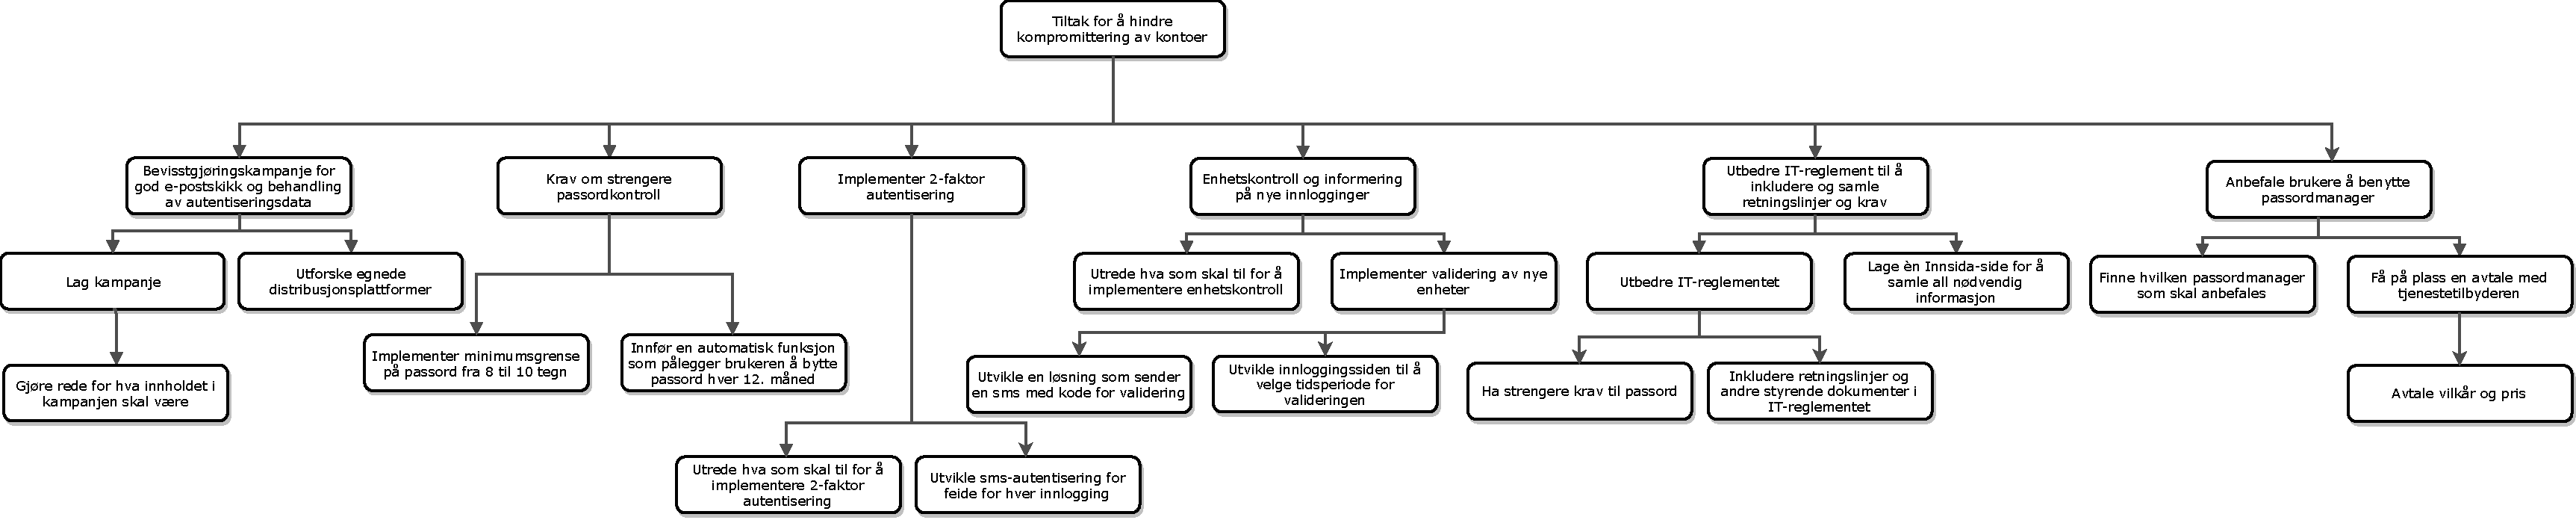
\includegraphics[scale=0.4, angle=90]{case_2/bilder/trediagram.pdf}
    \caption[Trediagram av tiltak mot kompromitterte kontoer]{Trediagram av tiltak mot kompromitterte kontoer}
    \label{fig:trediagram-case2}
\end{figure}

\section{Kostnad-nytte-analyse}
\label{kost-nytte-case2}
Denne seksjonen tar for seg en kostnad-nytte-analyse av nytteverdien til bruk av rotårsaksanalyse for case 2. 

\subsection{Kostnad for gjennomføring}
I denne analysen definerer vi kostnad som tid brukt på en iterasjonen av metoden. Vi definerer en skala for kostnad fra 1 til 5 der nivåene tilsvarer følgende tidsbruk:

\begin{enumerate}
    \item Under 50 timer
    \item 50-150 timer
    \item 150-250 timer
    \item 250-400 timer
    \item Over 400 timer
\end{enumerate}

Tabell \ref{tab:tidsbruk_case2} under viser tidsbruken i enkeltfasene i dette caset. Dette inkluderer tid brukt til å dokumentere alt som har med de enkelte fasene å gjøre. 

% Table generated by Excel2LaTeX from sheet 'Ark1'
\begin{table}[H]
  \centering
  \caption{Tidsbruk i de ulike fasene i case 2}
    \begin{tabular}{|lr|l|}
    \hline
    \multicolumn{3}{|c|}{\cellcolor{yellow}\textbf{Case 2}} \\
    \hline
    \multicolumn{1}{|l|}{\cellcolor{apricot}\textbf{Fase}} & \multicolumn{1}{l|}{\cellcolor{apricot}\textbf{Verktøy brukt}} & \cellcolor{apricot}\textbf{Timer totalt} \\
    \hline
    \multicolumn{1}{|l|}{Problemforståelse} & \multicolumn{1}{l|}{Kritiske hendelser} & 14-18t \\
    \hline
    \multicolumn{1}{|l|}{Idémyldring} & \multicolumn{1}{l|}{Idemyldring} & 14-18t \\
    \hline
    \multicolumn{1}{|l|}{Datainnsamling} & \multicolumn{1}{l|}{Sampling og spørreundersøkelse} & 70-90t \\
    \hline
    \multicolumn{1}{|l|}{Datanalyse} & \multicolumn{1}{l|}{Analyseverktøy} & 90-110t \\
    \hline
    \multicolumn{1}{|l|}{Rotårsaksidentifisering} & \multicolumn{1}{l|}{Årsak-virkningsdiagram og 5 Whys} & 18-22t \\
    \hline
    \multicolumn{1}{|l|}{Rotårsakseliminering} & \multicolumn{1}{l|}{SIT} & 14-18t \\
    \hline
    \multicolumn{1}{|l|}{Løsningsimplementering} & \multicolumn{1}{l|}{Trediagram} & 8-10t \\
    \hline
    \multicolumn{2}{|l|}{\textbf{Sum}} & \textbf{228-286t} \\
    \hline
    \end{tabular}%
  \label{tab:tidsbruk_case2}%
\end{table}%

Dersom kosten på caset går over flere nivåer regner vi med medianen til ytterpunktene for å plassere kostnaden. Basert på kostnadsnivåene vi definerte over, plasseres tidsbruken på case 2 til:
\[Kostnad = 4\]

\subsection{Nytte av resultatene}
I denne analysen definerer vi nytten som egen oppfatning av hvor gode resultatene fra caset var. Det vurderes ut fra om vi tror det kan finnes andre underliggende årsaker, og hvorvidt vi mener problemet blir løst dersom rotårsakene fjernes. Nytten defineres på en skala fra 1 til 5. 

I dette caset kom vi frem til at rotårsakene var spredt over flere årsaker. Hovedårsakene var gjenbruk av kredentialier på flere tjenester, phishing og utilstrekkelig tilgangskontroll på brukerkontoene. Vi er sikre på at hvis disse årsakene fjernes, vil brorparten av problemet løses. Vi definerer derfor nytten til:
\[Nytte = 5\]

\subsection{Total nytteverdi}
Når vi regner ut kostnad-nytte deler vi kostnaden på nytteverdien. 
\[\frac{Kostnad}{Nytte} = Total nytteverdi\]

I dette caset blir regnestykket slik:
\[\frac{4}{5} = 0,8\]

Svarene på regnestykket kan bli fra 0,2 til 5. Jo lavere denne nytteverdien er, jo bedre fungerte metoden til caset. 